\title{Monografia - Kevin}

\documentclass[
	% -- opções da classe memoir --
	12pt, % tamanho da fonte
    oneside, % Tipo de impressão, frente-verso(twoside) ou apenas frente(oneside)
	a4paper, % tamanho do papel. 
	% -- opções da classe abntex2 --
	chapter=TITLE, % títulos de capítulos convertidos em letras maiúsculas
	% -- opções do pacote babel --    
	english, % idioma adicional para hifenização
	brazil % o último idioma é o principal do documento    
	]{abntex2}
    
    %\renewcommand{\ABNTEXpartfontsize}{\normalsize}
	%\renewcommand{\ABNTEXchapterfontsize}{ \large}
	%\renewcommand{\ABNTEXsectionfontsize}{\normalsize}
	%\renewcommand{\ABNTEXsubsectionfontsize}{\normalsize}

% ---
% Pacotes básicos 
% ---
\usepackage{lmodern} % Usa a fonte Latin Modern			
\usepackage[T1]{fontenc} % Selecao de codigos de fonte.
\usepackage[utf8]{inputenc} % Codificacao do documento (conversão automática dos acentos)
\usepackage{lastpage} % Usado pela Ficha catalográfica
\usepackage{indentfirst} % Indenta o primeiro parágrafo de cada seção.
\usepackage{color} % Controle das cores
\usepackage{graphicx} % Inclusão de gráficos
\usepackage{microtype} % para melhorias de justificação
\usepackage{todonotes}
\usepackage{tabularx}
\renewcommand{\tabularxcolumn}[1]{m{#1}}
\usepackage{pdflscape}

\definecolor{algColor}{RGB}{255,206,206} % rgb(255, 206, 206)

% Pacotes para algoritmos/pseudo-código
\usepackage{listings}

\renewcommand{\lstlistingname}{Programa}

\lstset
{ %Formatting for code in appendix
    language=C,
    basicstyle=\footnotesize,
    numbers=left,
    stepnumber=1,
    frame = single,
    showstringspaces=false,
    tabsize=2,
    breaklines=true,
    xleftmargin=10pt,
    breakatwhitespace=false,
    extendedchars=true,
    literate={á}{{\'a}}1 
             {ã}{{\~a}}1
             {é}{{\'e}}1
             {í}{{\'i}}1
             {õ}{{\~o}}1
             {ç}{{\c{c}}}1,
}
\lstset{language=VHDL}
\renewcommand{\lstlistlistingname}{Lista de códigos}

% Configura a ``Lista de Códigos'' conforme as regras da ABNT (para abnTeX2)
\begingroup\makeatletter
\let\newcounter\@gobble\let\setcounter\@gobbletwo
  \globaldefs\@ne \let\c@loldepth\@ne
  \newlistof{listings}{lol}{\lstlistlistingname}
  \newlistentry{lstlisting}{lol}{0}
\endgroup

\renewcommand{\cftlstlistingaftersnum}{\hfill--\hfill}

\let\oldlstlistoflistings\lstlistoflistings
\renewcommand{\lstlistoflistings}{%
   \begingroup%
   \let\oldnumberline\numberline%
   \renewcommand{\numberline}{\lstlistingname\space\oldnumberline}%
   \oldlstlistoflistings%
   \endgroup}
% ---
% Pacotes adicionais, usados apenas no âmbito do Modelo Canônico do abnteX2
% ---
\usepackage{lipsum} % para geração de dummy text
% ---
% ---
% Pacotes de citações
% ---
\usepackage[alf, % Citações Autor-Data
    abnt-etal-cite=2,  % ``et. al'' a partir de 3 autores nas citações
    abnt-etal-list=0,  % tirar ``et. al'' a partir de 4 autores nas referências
    abnt-emphasize=bf  % Enfatizar o título da publicação com negrito
]{abntex2cite}

% --- 
% CONFIGURAÇÕES DE PACOTES
% --- 

\usepackage{abntex_ufrr_dcc}

% PACOTES DE ALGORITMO

\usepackage{algpseudocode,algorithm}
% Declaracoes em Português

\algrenewcommand\algorithmicend{\textbf{FIM}}
\algrenewcommand\algorithmicdo{\textbf{FAÇA}}
\algrenewcommand\algorithmicwhile{\textbf{ENQUANTO}}
\algrenewcommand\algorithmicfor{\textbf{PARA}}
\algrenewcommand\algorithmicforall{\textbf{PARA TODO}}
\algrenewcommand\algorithmicif{\textbf{SE}}
\algrenewcommand\algorithmicthen{\textbf{ENTÃO}}
\algrenewcommand\algorithmicelse{\textbf{SENÃO}}
\algrenewcommand\algorithmicreturn{\textbf{RETORNE}}
\algrenewcommand\algorithmicfunction{\textbf{FUNÇÃO}}
% New definitions
\algnewcommand\algorithmicswitch{\textbf{ESCOLHA}}
\algnewcommand\algorithmiccase{\textbf{CASO}}
\algnewcommand\algorithmicassert{\texttt{assert}}
\algnewcommand\Assert[1]{\State \algorithmicassert(#1)}%
% New "environments"
\algdef{SE}[SWITCH]{Switch}{EndSwitch}[1]{\algorithmicswitch\ #1\ \algorithmicdo}{\algorithmicend\ \algorithmicswitch}%
\algdef{SE}[CASE]{Case}{EndCase}[1]{\algorithmiccase\ #1}{\algorithmicend\ \algorithmiccase}%
\algtext*{EndSwitch}%
\algtext*{EndCase}%


% Rearranja os finais de cada estrutura
\algrenewtext{EndWhile}{\algorithmicend\ \algorithmicwhile}
\algrenewtext{EndFor}{\algorithmicend\ \algorithmicfor}
\algrenewtext{EndIf}{\algorithmicend\ \algorithmicif}
\algrenewtext{EndFunction}{\algorithmicend\ \algorithmicfunction}

% O comando For, a seguir, retorna 'para #1 -- #2 até #3 faça'
\algnewcommand\algorithmicto{\textbf{até}}
\algrenewtext{For}[3]%
{\algorithmicfor\ #1 $\gets$ #2 \algorithmicto\ #3 \algorithmicdo}


% ---
% Configurações do pacote backref
% Usado sem a opção hyperpageref de backref
%\renewcommand{\backrefpagesname}{Citado na(s) página(s):~}
% Texto padrão antes do número das páginas
%\renewcommand{\backref}{}
% Define os textos da citação
%\renewcommand*{\backrefalt}[4]{
%	\ifcase #1 %
%		Nenhuma citação no texto.%
%	\or
%		Citado na página #2.%
%	\else
%		Citado #1 vezes nas páginas #2.%
%	\fi}%
% ---

% ---
% Informações de dados para CAPA e FOLHA DE ROSTO
% ---
\titulo{\textbf{VERIFICAÇÃO FORMAL DE CIRCUITOS LÓGICOS BASEADOS EM TRANSFORMAÇÃO DE CÓDIGO COM \textit{BOUNDED MODEL CHECKING}}}

\autor{KEVIN COSTA AIRES OLIVEIRA}
\local{Boa Vista - RR}
\data{2018}
\orientador{Dr. Herbert Oliveira Rocha}

\tipotrabalho{Monografia}

\preambulo{Monografia de Graduação apresentada ao Departamento de Ciência da Computação da Universidade Federal de Roraima como requisito parcial para a obtenção do grau de Bacharel em Ciência da Computação.}

%Trabalho de conclusão de curso  na área de Verificação de Software desenvolvido na UFRR com o %objetivo \textcolor{red}{VERIFICAR O PADRÃO DOS OUTROS TCC} de gerar casos de teste para %sistemas embarcados críticos
% ---
%-- Informações de dado para a FOLHA DE APROVAÇÃO
\renewcommand{\dataDefesa}{01 de Fevereiro de 2018}
\renewcommand{\orientadorBanca}{Prof. Dr. Herbert Oliveira Rocha}
\renewcommand{\primeiroMembroBanca}{Prof. Me. Acauan Cardoso Ribeiro}
\renewcommand{\segundoMembroBanca}{Prof. Me. Filipe Dwan Perreira}

% ---
% Configurações de aparência do PDF final

% alterando o aspecto da cor azul
\definecolor{blue}{RGB}{41,5,195}

% informações do PDF
\makeatletter
\hypersetup{
     	%pagebackref=true,
		pdftitle={\@title}, 
		pdfauthor={\@author},
    	pdfsubject={\imprimirpreambulo},
	    pdfcreator={LaTeX with abnTeX2},
		pdfkeywords={abnt}{latex}{abntex}{abntex2}{trabalho acadêmico}, 
		colorlinks=true, % false: boxed links; true: colored links
    	linkcolor=blue, % color of internal links
    	citecolor=blue, % color of links to bibliography
    	filecolor=magenta, % color of file links
		urlcolor=blue,
		bookmarksdepth=4
}
\makeatother
% --- 
% --- 
% Espaçamentos entre linhas e parágrafos 
% --- 
% O tamanho do parágrafo é dado por:
\setlength{\parindent}{1.3cm}
% Controle do espaçamento entre um parágrafo e outro:
\setlength{\parskip}{0.2cm}  % tente também \onelineskip
% ---
% compila o indice
% ---
\makeindex
% ----
% ----
% Início do documento
% ----
\begin{document}
% Retira espaço extra obsoleto entre as frases.
\frenchspacing 
% ----------------------------------------------------------
% ELEMENTOS PRÉ-TEXTUAIS
% ----------------------------------------------------------
% \pretextual
% ---
% Capa
% ---
\imprimircapa
% ---
% ---
% Folha de rosto
% (o * indica que haverá a ficha bibliográfica)
% ---
\imprimirfolhaderosto
% ---
% ---
% Inserir folha de aprovação
% ---
\imprimirfolhadeaprovacao
% ---
% Dedicatória
% ---
\begin{dedicatoria}
   \vspace*{\fill}
   \centering
   \noindent
   \textit{Dedico este trabalho a minha familia e amigos e a todos aqueles que acreditaram no meu esforço. } \vspace*{\fill}
\end{dedicatoria}
% ---
% ---
% Agradecimentos
% ---
\begin{agradecimentos}[Agradecimentos]
\par
Primeiramente, agradeço a minha família, por sempre está ao meu lado nos momentos mais difíceis da faculdade, pelos conselhos e pelo o incentivo em todos estes anos de faculdade.
\par
Agradeço ao meu orientador, professor Herbert Oliveira, por todo apoio desde a disciplina de arquitetura de computadores, por todas as orientações no desenvolvimento deste projeto, além dos incentivos para vida pós faculdade.
\par
Agradeço também aos amigos que sempre ajudaram, seja lendo uma lauda por cada encontro, discutindo sobre seções no laboratório ou na sala, fazendo companhia em algum posto, incentivando e corrigindo os erros de português. 
\par
Agradeço aos professores do DCC que durantes estes anos de curso foram fonte de aprendizado e incentivos durante aulas e que cada uma pode contribuir de alguma forma no meu desenvolvimento como aluno e futuro profissional.
\end{agradecimentos}
% ---
% ---
% Epígrafe
% ---
\begin{epigrafe}
    \vspace*{\fill}
	\begin{flushright}
		\textit{Não importa o que o mundo diz de mim, o que importa é que eu nunca fiz nada que contrariasse os meus princípios e nunca farei.}
	\end{flushright}
\end{epigrafe}
% ---
% ---
% RESUMOS
% ---
% resumo em português
\setlength{\absparsep}{18pt} % ajusta o espaçamento dos parágrafos do resumo
\begin{resumo}[Resumo]
O objetivo desse trabalho é a verificação de circuitos lógicos descritos em VHDL, adotando técnicas de verificação formal e transformações de código, buscando identificar funcionamento incorreto de determinado circuito. A análise é realizada através da inserção de assertivas contendo propriedades sobre um dado circuito analisado em VHDL, onde é aplicada transformação e instrumentação de código VHDL para C para utilização da técnica de indução-k para exploração dos estados alcançáveis do circuito e assim determinar a ocorrência ou não de violação de propriedade descrita na assertiva inserida ao código. Para etapa de tradução foi desenvolvido dois métodos de tradução, buscando a melhor tradução, através de uma única ferramenta ou através de várias ferramentas. Para a análise foi utilizada a mesma ferramenta, chamada ESBMC (\textit{Extended SMT-Based Bounded Model Checker}) que utilizou a técnica de indução-k para análise de todos os códigos. A ferramenta utilizou as pré e pós condições inseridas em cada código para analisar se elas foram violadas ou não.
%Durante os teste iniciais, foi desenvolvido uma ferramenta para automatizar o método proposto, onde foi constatado que a ferramenta de tradução de código VHDL para C apresentava limitações em relação as estruturas em VHDL, de modo a evitar que circuitos mais complexos pudessem ser analisados e assim restringindo a capacidade do método proposto neste trabalho. Positivamente, a ferramenta de BMC adotada, neste caso o ESBMC (\textit{Extended SMT-Based Bounded Model Checker}) apresentou resultados positivos, ou seja, validando as assertivas/propriedades de forma correta. 
Como trabalhos futuros, a inserção automática das assertivas torna o método mais independente do desenvolvedor, por tem uma menor carga de interferência. Também refinar ainda mais a tradução, buscando abranger cada vez mais elementos da linguagem VHDL.
\vspace{\onelineskip}
\noindent
\par
\textbf{Palavras-chaves}: Transformação de código, Bounded Model Cheching, VHDL, Hardware, Assertivas.
\end{resumo}
% \begin{resumo}[Abstract]
% \begin{otherlanguage*}{english}
   Fazer Abstract!!

\vspace{\onelineskip}
\noindent 
\textbf{Key-words}: ??
\end{otherlanguage*}
% \end{resumo}
% ---
% inserir lista de ilustrações
% ---
\pdfbookmark[0]{\listfigurename}{lof}
\renewcommand{\listfigurename}{Lista de Figuras}
\listoffigures*
\cleardoublepage
% ---
% ---
% inserir lista de tabelas
% ---
\pdfbookmark[0]{\listtablename}{lot}
\renewcommand{\listtablename}{Lista de Tabelas}
\listoftables*
\cleardoublepage
% ---
% ---
% inserir lista de abreviaturas e siglas
% ---
% \begin{siglas}
%   \item[BMC] Bounded Model Checking
%   \item[ESBMC] Efficient SMT-Based Context-Bounded Model Checker
%   \item[HDL] Hardware Description Language
%   \item[PSL] Property Specification Language
%   \item[SE] Sistemas Embarcados
%   \item[VHDL] VHISIC Hardware Description Language
% \end{siglas}
% ---
% ---
% inserir lista de símbolos
% ---
% \begin{simbolos}  
%   \item[$ \Gamma $] \todo{Atualizar esta lista!} Letra grega Gama
%   \item[$ \Lambda $] Lambda
%   \item[$ \zeta $] Letra grega minúscula zeta
%   \item[$ \in $] Pertence
% \end{simbolos}
% % ---
% ---
% inserir o sumario
% ---
\pdfbookmark[0]{\contentsname}{toc}
\renewcommand{\contentsname}{Sumário}
\tableofcontents*
\cleardoublepage
% ---
%--------------------------------------------------------
% ELEMENTOS TEXTUAIS
%--------------------------------------------------------
\textual
%--------------------------------------------------------
% Introdução
%--------------------------------------------------------
\chapter{INTRODUÇÃO}
%\textcolor{red}{A complexidade de sistemas computacionais cresce exponencialmente.} \todo{Exemplificar este crescimento.Pesquisar sobre o facebook} 
%Muitas companhias e organizações estão rotineiramente lidando com software que contém milhares de linhas de código, escritos por diferentes pessoas, que usam linguagens distintas, ferramentas, estilos e hardware projetados de diversas formas e combinações \cite{hoder2011case}. 

\par
No contexto de sistemas compostos de hardware e software, tem-se os sistemas embarcados (SE) que são dispositivos semicondutores com software integrados, os quais se conectam a outros dispositivos. Usualmente, o principal propósito de um SE é o controle e provimento de informações para uma função específica \cite{ramesh2012energy}. 

\par
%Os SE são extremamente interativos com seu ambiente, operam geralmente em tempo real e estão disponíveis continuamente. No entanto, estes sistemas, por possuírem um curto espaço de tempo para a liberação do produto ao mercado, precisam ser desenvolvidos rapidamente e atingir um alto nível de qualidade, mas, devido a esta necessidade, os programadores podem cometer enganos durante a fase de desenvolvimento destes sistemas.

\par
Os SE têm se proliferado em partes consideráveis das atividades do nosso cotidiano, com a característica de possuir grande quantidade de complexidade e diversidade. Devido a esta complexidade, erros podem passar despercebidos, causando não apenas penalidades econômicas e/ou fracassos do produto no mercado, mas principalmente o risco de perda de vidas humanas \cite{cabodi2016hardware}. Como, por exemplo, o acidente noticiado no \cite{g1Acidente}, no qual, de acordo com o secretário de transportes, uma falha na placa do circuito eletrônico responsável pelo controle de velocidade dos trens ocasionou a colisão entre duas composições na estação de metrô de São Paulo.

\par
Segundo \citeonline{rocha2015verificaccao}, para se obter um alto nível de qualidade no desenvolvimento dos sistemas de hardware e software, a execução desses sistemas deve ser controlada e da mesma forma deve-se buscar meios de garantir que as propriedades definidas sejam atingidas. Por exemplo, a partir do conhecimento prévio do modo de implementação de determinado hardware, é possível utilizá-lo de forma mais eficiente. Neste sentido, diversas estratégias de verificação e de teste estão sendo pesquisadas e aplicadas para garantir a qualidade do software e hardware \cite{hoder2010interpolation,rocha2010exploiting,brayton2010abc,cordeiro2012smt,cabodi2016hardware}.

\par
Por este motivo, com o intuito de analisar e otimizar a descrição dos circuitos digitais, tem-se utilizado as linguagens de descrição de hardware (HDL). Estas se diferem das linguagens de programação por conseguirem gerar execuções não apenas sequenciais, como também concorrentes ou paralelas \cite{chu2006rtl}.
% 
% \par
Neste contexto, a \textit{VHSIC Hardware Description Language} (VHDL) é uma das linguagens de descrição de hardware mais utilizadas atualmente. A descrição em VHDL pode ser em vários níveis de abstração, sendo o mais alto o nível comportamental que permite a descrição do circuito através de \textit{loops} e processos, definido-o na forma de algoritmo. Como características das linguagens de descrição, o VHDL permite declarações sequenciais ou concorrentes onde as declarações continuam ativas e sua ordem torna-se irrelevante \cite{cappelattipraticando}.

\par
Aliada à linguagem de descrição de hardware, a  verificação formal de sistemas computacionais tem desempenhado um papel importante para assegurar a previsibilidade e a confiabilidade na concepção de aplicações críticas. E, para isso, tem-se utilizado a técnica denominada \textit{model checking}, que é baseada em formalismos matemáticos para provar propriedades de programas reativos \cite{bensalem1999automatic}. Esta técnica gera uma busca exaustiva no espaço de estados do modelo para determinar se uma dada propriedade é válida ou não \cite{baier2008principles}, tendo como principal razão para o seu sucesso o funcionamento completamente automático, ou seja, sem qualquer intervenção do usuário.

\par
Visando contribuir com verificação de sistemas computacionais, principalmente, no âmbito de sistemas embarcados, o contexto deste trabalho está situado no uso de metodologias e técnicas de verificação formal para programas escritos em VHDL \cite{biere2016aiger}, focando principalmente no \textit{Bounded Model Checking} \cite{cordeiro2012smt,rocha2015model}. Este trabalho está interessado especificamente na parte de verificação de modelos de hardware descritos em níveis de circuitos de bits na linguagem VHDL, via transformações de código para gerar modelos, com assertivas, já suportados por \textit{model checkers}, como o ESBMC \cite{cordeiro2012smt}. 

\par
Dessa forma, o trabalho almeja analisar as propriedades de alcançabilidade para a identificação de localizações de erro, bem como, assertivas contendo propriedades de segurança. A propriedade de alcançabilidade ou propriedade do estado de erro é satisfatória (SAT), se um estado de erro é alcançável. Caso contrário, a propriedade é considerada insatisfatória (UNSAT). No caso SAT, o \textit{model checking} também gera um rastreio da validação da propriedade (contra-exemplo), ou seja, uma sequência de estados que mostra como chegar ao erro a partir de um ponto inicial.

%===========================================================
%DEFINIÇÃO DO PROBLEMA
%===========================================================
\section{Definição do problema}

O avanço da tecnologia, principalmente nas áreas de design e fabricação de eletrônicos, aumentou a importância do hardware nos dias atuais. Cada vez com mais funcionalidades integradas, aliada a velocidade e circuitos menores, faz com que a complexidade dos sistemas de hardware aumente. Entretanto, por este motivo, a detecção tardia de erros no sistema pode resultar em perda de produção, mas também custos associados ao desenvolvimento do sistema \cite{gupta1992formal}. Sendo assim, a verificação de hardware visa assegurar que o circuito atinja as especificações para o qual foi projetado, através de técnicas formais ou dinâmicas \cite{boule2007efficient}.

%Os erros durante o desenvolvimento de sistemas computacionais %tornaram-se mais comuns, em parte devido ao curto espaço de tempo de %sua liberação. Logo, é necessário que as aplicações sejam projetadas %considerando os requisitos de previsibilidade e confiabilidade, %principalmente em aplicações de sistemas embarcados críticos, onde %diversas restrições (por exemplo, tempo de resposta e precisão dos %dados) devem ser atendidas e mensuradas de acordo com os requisitos %do usuário, caso contrário uma falha pode conduzir a situações %catastróficas. 
\par
Por esta razão, a utilização de métodos formais tornou-se uma abordagem atraente para superar as limitações inerentes à validação baseada em simulação. Portanto, a maioria das empresas de semicondutores têm investigado a sua aplicabilidade. Escolhas individuais de métodos, ferramentas e áreas de aplicação das empresas têm variado, assim como o seu nível de sucesso~\cite{cabodi2016hardware}. Com os recentes avanços na escalabilidade de automação dos \textit{model checkers} e nas equivalências sequenciais de verificação, a maioria das empresas têm crescido ao contar com essas técnicas\cite{clarke2008birth}.

\par 
O problema considerado neste trabalho é expresso na seguinte questão: \textbf{Como complementar e aprimorar a verificação de propriedades de segurança em circuitos lógicos, de tal forma que uma propriedade possa ser mapeada em um problema de alcançabilidade simbólica, ou seja, é possível alcançar um estado específico (para uma dada propriedade) a partir do estado inicial?}

%===========================================================
%OBJETIVOS GERAIS E ESPECIFICOS
%===========================================================
\section{Objetivos}

O objetivo principal deste trabalho é projetar e avaliar um método para efetuar a verificação de circuitos descritos em VHDL com portas lógicas em nível de bit pela utilização de técnicas de transformação de códigos combinado com a técnica \textit{Bounded Model Checking} para exploração de estados alcançáveis no circuito, visando identificar erros ou comportamentos indevidos ou inesperados que podem resultar no funcionamento incorreto de um dado sistema.

Os objetivos específicos são:
\begin{enumerate}
  \item Propor um método para especificar pré e pós-condições de circuitos digitais em nível de portas lógicas descritos em VHDL;
  \item Analisar ferramentas de verificação de modelos que utilizam a técnica \textit{Bounded Model Checking};
  \item Especificar uma técnica de conversão de circuitos em linguagem de descrição de hardware VHDL para um modelo a ser verificado usando a técnica \textit{Bounded Model Checking};
   \item Desenvolver um método para identificação de estados de erros ou ocorrências indevidas, de um dado circuito analisado, em modelos de hardware descritos em nível de bit na linguagem de descrição VHDL.
  \item Validar a aplicação do método proposto sobre \textit{benchmarks} públicos de programas em VHDL, a fim de examinar a sua eficácia e aplicabilidade.
\end{enumerate}

%===========================================================
%METODOLOGIA PROPOSTA
%===========================================================
% \section{Metodologia proposta}
% 
%Esta seção descreve as principais etapas que foram identificadas para alcançar os objetivos deste trabalho. Estas etapas fornecem os passos necessários e direções para desenvolver a metodologia proposta e podem ser descrita em três diferentes fases como segue: análise do domínio, metodologia proposta e validação da metodologia.
% 
% Na etapa de análise de domínio, toda a teoria necessária para entender os métodos, técnicas e ferramentas aplicadas à metodologia de desenvolvimento/validação de circuitos lógicos utilizando a linguagem de descrição de hardware VHDL serão analisadas e avaliadas. Na fase da metodologia proposta, uma versão inicial da metodologia para verificação de circuitos lógicos, tem como foco uma ou mais restrições, e seu escopo serão precisamente definidos e propostos. Depois disso, esta metodologia é mais adiante refinada na fase de validação aplicando-a na verificação dos estudos de caso.
% 
% Com o intuito de realizar as atividades deste trabalho, uma abordagem iterativa e incremental será usada com o propósito de reduzir riscos e incertezas. Sendo assim, para cada incremento da solução proposta, as três etapas nomeadas nesta proposta como análise do domínio, metodologia proposta e validação da metodologia podem ser tratadas com diferentes ênfases em cada fase do trabalho.
% 
% Por exemplo, no início deste trabalho, a análise de domínio provavelmente terá maior ênfase do que as outras fases metodologia proposta e validação da metodologia. Na metade do projeto, a fase de metodologia proposta provavelmente terá mais ênfase do que as outras duas fases. Finalmente, a fase de validação da metodologia provavelmente terá mais ênfase no fim do desenvolvimento deste TCC. A principal razão para adotar uma abordagem iterativa e incremental é desenvolver o TCC incrementalmente, permitindo assim tirar vantagem do que foi aprendido durante cada incremento do projeto.
% 
% % Para cada incremento do TCC, relatórios técnicos devem ser escritos com o propósito de descrever os principais feitos alcançados em uma dada iteração. Além disso, se os resultados significantes têm sido alcançados, então artigos científicos podem ser escritos para reportá-los à comunidade acadêmica através das publicações em workshops e conferências nacionais/internacionais. Potencialmente, os artigos científicos podem ser produzidos em cada incremento do projeto com o intuito de fornecer claramente o progresso deste projeto de pesquisa.

%===========================================================
%CONTRIBUIÇÕES PROPOSTAS
%===========================================================
% \section{Contribuições propostas}
% 
% As contribuições propostas para este trabalho são:
% \begin{itemize}
%   \item O desenvolvimento de um método para verificação de hardware com o intuito de facilitar os passos da verificação e ao mesmo tempo reduzir substancialmente o tempo de verificação de projetos de hardware descritos em VHDL;
%   \item Este trabalho apresenta para o método proposto, o desenvolvimento e implementação de uma ferramenta de verificação de circuitos lógicos em VHDL com a integração da ferramenta ESBMC (\textit{Efficient SMT-Based Context-Bounded Model Checker})\cite{cordeiro2012smt} na análise.
% \end{itemize}

%===========================================================
%ORGANIZAÇÃO DO TRABALHO
%===========================================================
\section{Organização do trabalho}
A introdução deste trabalho apresentou: o contexto, definição do problema, e objetivos deste trabalho. Os próximos capítulos estão organizados da seguinte forma:

\par
No \autoref{chapter:conceitos} \textbf{Conceitos e Definições}, são apresentados os conceitos abordados neste trabalho, especificamente: Linguagens de descrição de hardware; Verificação e validação de sistemas; e Técnicas de compiladores.

\par
No \autoref{chapter:correlatos}, \textbf{Trabalhos Correlatos}, serão apresentados o método de pesquisa bibliográfica utilizado, sendo ele a revisão sistemática, seguido do resultado encontrado com esta pesquisa e, por fim, a contribuição dos artigos utilizados no desenvolvimento do projeto. 

\par
No \autoref{chapter:metodo}, \textbf{Método Proposto}, são descritas as etapas de execução do método proposto anterior, bem como o novo método a ser apresentado. Apresentar as diferenças entre os métodos e a causa das mudanças.

\par
No \autoref{chapter:resultados} \textbf{Resultados experimentais}, apresenta os testes realizados com as duas abordagens utilizadas, além de demonstrar os pontos que tiveram melhorias entre os dois os métodos.


\par
E, por fim, no \autoref{chapter:consideracoes}, \textbf{Considerações finais e trabalhos futuros}, serão apresentas as considerações finais, principais pontos levantados no desenvolvimento do trabaho e as sugestões de trabalhos futuros. 

%========================
%===Resumo do capitulo===
%========================
\section{Resumo do capitulo}
\par
Neste capitulo foi apresentado uma breve introdução e contextualizção, a definição do problema do projeto que consiste na verificação de propriedades de circuitos lógicos, os objetivos que entre eles se encontra o dsenvolvimento de um método para identificação de erros em circuitos lógicos e validação deste metodo. E por fim. apresenta a estrutura utilizada neste trabalho, composta por conceitos e definições, trabalhos correlatos, método proposto, resultados experimentais e considerações finais e trabalhos futuros.
%------------------------------------------------------------
% Conceitos e Definições
%------------------------------------------------------------
\chapter{CONCEITOS E DEFINIÇÕES}
\label{chapter:conceitos}
Este capítulo tem apresenta os principais conceitos e definições abordados neste trabalho, tais como: Linguagens de descrição de hardware, Verificação de sistemas e Técnicas de Compiladores.

%============================
%Linguagens de descrição de hardware
%============================
\section{Linguagens de descrição de hardware}

As linguagens de descrição de hardware (HDL) foram desenvolvidas com o intuito de auxiliar a criação de circuitos lógicos com grande número de elementos e com uma gama de abstrações lógicas e eletrônicas~\cite{thomas2008verilog}. \textcolor{red}{Entre os exemplos, podemos citar: \textit{VDHL}~\cite{IEEEVHDLLanguage}, \textit{Verilog}~\cite{IEEEVerilogLanguage} e \textit{SystemC}~\cite{IEEESystemCLanguage}.}

\par
Segundo~\cite{christen1999vhdl}, linguagens de descrição de hardware são linguagens de programação utilizadas com o intuito de descrever o comportamento de um determinado circuito, técnica conhecida como modelagem. Os modelos descritos em HDL são utilizados como entrada para um simulador, onde o mesmo pode ter seu comportamento analisado.

\par
As HDL's trazem consigo diversas vantagens, entre elas códigos independentes de tecnologia e fabricante, podendo ser portáteis e reutilizáveis \cite{cappelattipraticando}. As linguagens mais modernas, tais como VHDL e \textit{Verilog}, possuem suporte tanto a descrição do circuito propriamente dito, quanto ao comportamento que o mesmo deve exercer \cite{christen1999vhdl}.

\par
A \textit{Verilog}, como já citado, é uma linguagem de descrição de \textit{hardware} que fornece diversos níveis de abstração para desenvolvimento de sistemas digitais\cite{thomas2008verilog}. A linguagem foi desenvolvida para ser simples e efetiva nos diversos níveis de abstração incluindo o suporte ao desenvolvimento, verificação, síntese e testes de \textit{software}~\cite{IEEEVerilogLanguage}.

\begin{figure}[H]
\caption{\label{fig:mux_verilog} Exemplo de multiplexador descrito em Verilog.}
	\begin{center}
    \begin{minipage}{0.7\textwidth}
    \begin{lstlisting}       
primitive multiplexer (mux, control, dataA, dataB);
output mux;
input control, dataA, dataB;
endprimitive
\end{lstlisting}
    \end{minipage}
	\end{center}
    \legend{Fonte: Adaptado de~\cite{IEEEVerilogLanguage}.}
\end{figure}

\par
\textcolor{red}{Na \autoref{fig:mux_verilog} apresenta um exemplo de multiplexador descrito em \textit{Verilog} utilizando a estrutura de modelagem, chamada \textit{UDP} que permite a criação de novos primitivas para serem utilizada. Apresenta uma saída apenas(mux) e três entradas sendo uma de controle(control) e duas de dados(dataA e dataB).}

\par
A VHDL é uma linguagem de descrição de hardware amplamente utilizada, concebida na década de 80, devido uma necessidade do Departamento de Defesa dos Estados Unidos da América~\cite{cappelattipraticando}. Assim como a Verilog, esta linguagem também suporta o desenvolvimento, a verificação, a síntese, e os testes de \textit{hardware}~\cite{IEEEVHDLLanguage}.

\begin{figure}[H]
\caption{\label{fig:mux_vhdl} Exemplo de multiplexador descrito em VHDL.}
	\begin{center}
    \begin{minipage}{0.6\textwidth}
    \begin{lstlisting}       
library IEEE;
use IEEE.std_logic_1164.all;
use IEEE.std_logic_unsigned.all;
entity mux2x1 is
port (sel: in STD_LOGIC;
      a,b: in STD_LOGIC;
      y: out STD_LOGIC);
end mux2x1;

architecture dataflow of mux2x1 is begin
y <= (a AND NOT sel) OR (b AND sel);
end dataflow.
\end{lstlisting}
    \end{minipage}
	\end{center}
    \legend{Fonte: \cite{cappelattipraticando}.}
\end{figure}

\par
\textcolor{red}{Na \autoref{fig:mux_vhdl} está descrito um multiplexador de duas entradas descrito em VHDL, apresentando na parte inicial as bibliotecas e na entidade(entity) a declaração das variáveis utilizadas. Na arquitetura(architecture) apresenta o funcionamento do multiplexador, relacionando entradas e saídas conforme tenham sido declarados. Este conceitos serão melhor apresentados na \autoref{sec:vhdl_seção}.}

\par
\textcolor{red}{Conforme apresentado nas \autoref{fig:mux_verilog} e \autoref{fig:mux_vhdl}, ambas as linguagens apresentam diferenças no modelos de declaração e utilização para descrição de hardware. Para este trabalho foi escolhido a VHDL devido a linguagem apresentar um melhor escopo para análise, facilitando o trabalho de análise proposto para este projeto.}


%Ambas as linguagens apresentam similaridades, sendo a linguagem VHDL escolhida para este trabalho devido a linguagem apresentar maior gama de recursos tanto para o desenvolvimento quanto para o auxílio nos testes\todo{Apresentar um exemplo com referência}.


%============================
%VHDL
%============================
\subsection{\label{sec:vhdl_seção}VHSIC Hardware Description Language - VHDL}
\todo[inline]{Revisar textos e verificar a necessidade de mais exemplo}

VHDL é uma linguagem de descrição de hardware destinada a ser utilizada em todas as etapas da criação de sistemas eletrônicos, sendo elas: desenvolvimento; verificação; síntese; e, teste de circuitos~\cite{IEEEVHDLLanguage}.
% 
Segundo \cite{cappelattipraticando}, a VHDL apresenta três principais pilares: \textbf{abstração}, que consiste na descrição com diferentes níveis de detalhes; \textbf{modularidade}, que permite a divisão do projeto em vários blocos ou módulos para posterior interconexão; e \textbf{hierarquia}, \textcolor{red}{permite que módulos possam ser compostos por submódulos e, os mesmos tenham níveis de abstração diferentes, dependendo da necessidade do projeto.} Devido a esta versatilidade que a linguagem VHDL foi selecionada para o trabalho proposto.

\par
Segundo \cite{IEEEVHDLLanguage} é necessário um padrão para formatação da descrição em VHDL: \textit{Entity} (Pinos de entrada/saída) e \textit{Architecture} (Arquitetura). A \textit{Entity} ou entidade representa o bloco onde são declaradas as entradas e as saídas do circuito utilizadas em todo o sistema, conforme apresentado na \autoref{fig:biblioteca_entidade}. A \textit{Architecture} ou arquitetura, apresentado na \autoref{fig:arquitetura}, define a relação entre entradas e saídas declaradas na entidade, podendo tais especificações serem completas ou parciais. Assim como em outras linguagens, bibliotecas podem ser adicionadas, para que novas funções e atributos possam ser utilizados no projeto.

\begin{figure}[!htp]
\caption{\label{fig:biblioteca_entidade} Exemplo de declaração de bibliotecas e entidade.}
	\begin{center}
    \begin{minipage}{0.6\textwidth}
    \begin{lstlisting}       
library ieee;
use IEEE.STD_LOGIC_1164.ALL

ENTITY full_adder IS PORT(
	x1,x2,cin: in std_logic;
   S,count:out std_logic);
END full_adder;
\end{lstlisting}
    \end{minipage}
	\end{center}
    \legend{Fonte: Própria.}
\end{figure}

\begin{figure}[!htp]
\caption{\label{fig:arquitetura} Exemplo de declaração da arquitetura no VHDL.}
	\begin{center}
    \begin{minipage}{0.6\textwidth}
    \begin{lstlisting}       
ARCHITECTURE behavioral OF full_adder IS
BEGIN
	s<=x1 XOR x2 XOR cin;
    cout<=(x1 AND x2) OR (x1 AND cin) OR (b AND cin);
END behavioral;

\end{lstlisting}
    \end{minipage}
	\end{center}
    \legend{Fonte: Própria.}
\end{figure}



Segundo \cite{cappelattipraticando}, uma descrição em VHDL pode conter diferentes níveis de abstração:
\begin{itemize}
  \item \textbf{Comportamental:} Permite descrever o circuito através de laços e processos. O circuito é definido em forma de um algoritmo, utilizando construção similares as utilizadas em linguagem de programação.
  
  \item \textbf{Transferência de registradores:} Englobando a representação do dispositivo em nível de transferência entre registradores, que consiste na utilização de funções lógicas combinacionais e de registradores.
  
  \item \textbf{Estrutural:} O circuito é descrito mais próximo da implementação real, podendo ser definidas portas lógicas com atrasos unitários ou com atrasos detalhados.
\end{itemize}


%============================
%PORTAS LÓGICAS
%============================
\subsection{Portas lógicas}

Segundo \citeauthor{idoeta1982elementos}\todo{Citação incorreta} o conceito de portas lógicas é baseado na conhecida álgebra de Boole ou álgebra booleana, desenvolvida pelo matemático inglês George Boole em 1854. A álgebra booleana é representada por apenas dois valores, sendo eles o $0$ e $1$ e, através disso, expressa a relação entre entrada e saída dentro de um circuito. As portas lógicas podem ser construídas a partir de diodos, \textcolor{red}{transistores} e resistores interconectados de modo que a saída seja o resultante de uma operação lógica básica realizada sobre as entradas \cite{tocci2003sistemas}. A \autoref{fig:algebra_booleana} apresenta um exemplo de álgebra booleana sem a utilização de diagramas.

\begin{figure}[!htbp]
	\begin{center}
    \caption{\label{fig:algebra_booleana}Exemplo de algebra booleana, onde A=0, B=1, C=1 e D=1.}
	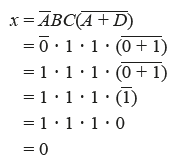
\includegraphics[scale=0.70]{Figuras/algebra_booleana.png}
	\end{center}
    \legend{Fonte: \cite{tocci2003sistemas}}
\end{figure}

\par
Ainda segundo \citeauthor{tocci2003sistemas}, devido a esta característica, a álgebra booleana possui três operações básicas, \textit{OR} (ou), \textit{AND} (e) e \textit{NOT} (não). Tal conjunto de operações também é denominado de operações booleanas e, por meio da utilização de tabelas verdade é possível descrever as saídas baseando-se nas entradas e na operação aplicada. Cada operação booleana possui sua tabela verdade (~\autoref{fig:exemplo_diagrama}), bem como sua representação em forma de diagrama.

\begin{figure}[H]
	\begin{center}
    \caption{\label{fig:exemplo_diagrama}Símbolo e tabela verdade para uma porta OR de três entradas.}
	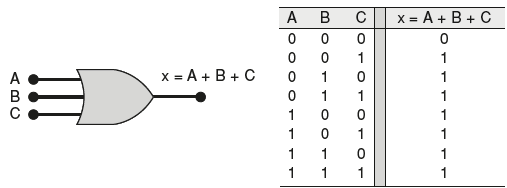
\includegraphics[scale=0.60]{Figuras/exemplo_diagrama.png}
	\end{center}
    \legend{Fonte: \cite{tocci2003sistemas}}
\end{figure}

\begin{figure}[H]
	\begin{center}
    \caption{\label{fig:exemplo_circuito} Representação de circuito lógico, utilizando portas lógicas.}
	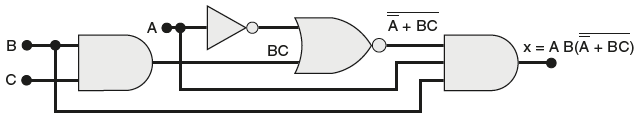
\includegraphics[scale=0.60]{Figuras/exemplo_circuito.png}
	\end{center}
    \legend{Fonte: \cite{tocci2003sistemas}}
\end{figure}

A \autoref{fig:exemplo_circuito} apresenta um circuito lógico formado pelas portas básicas da álgebra booleana. O circuito apresenta três entradas representadas pelas letras A, B e C, mas também formada por duas portas \textit{AND}, uma porta \textit{NOT} e uma porta \textit{OR}. Cada uma destas portas representando operações a serem realizadas, podendo receber como entrada um valor inicial ou resultante de outra porta, como no exemplo ocorre com a última porta \textit{AND}.

\todo[inline]{Adicionar um exemplo para apresentar a dificuldade de explorar todas as possibilidades de um circuito}

\todo[inline]{Falar sobre o problema da satisfabilidade NPC}

%============================
%VERIFICAÇÃO DE SISTEMAS
%============================
\section{Verificação de sistemas}
 No contexto de verificação de sistemas, faz-se necessário a diferenciação entre verificação e validação. Verificação e validação possuem o intuíto de mostrar que determinado sistema funcione conforme o especificado, além de satisfazer as especificações do cliente~\cite{sommerville2011engenharia}. 

\par
Segundo~\cite{sargent2005verification}, verificação é o processo de determinar se um modelo computacional obtido por discretização de um modelo matemático de um evento físico e o código que implementa o modelo computacional pode ser usado para representar o modelo matemático do evento com precisão suficiente e validação é o processo de determinar se um modelo matemático de um evento físico representa o evento físico real com precisão suficiente.

\par
A verificação consite identificação de erros e provavéis problemas que um componente pronto possa apresentar, enquanto a validação busca analisar se tal componete esta seguindo os requisitos pré-definidos para sua construção~\cite{koscianski2007qualidade}. O teste de programa, na qual o software  é executado com dados de teste é a principal forma de validação, porém, tecnicas de verificação, tais como, inspeção e revisões também podem integrar a etapa de validação~\cite{sommerville2011engenharia}.

\subsection{Diagrama de decisão binária}
Um diagrama de decisão binária pode ser definido como um grafo aciclico para representação de funcões boolenas. Existe uma ordem rigorosa na ocorrência de variáveis à medida que se percorre o grafo da raiz para a folha. Dado como exemplo a formula \textit{f=(a$\lor$b)$\land$(c$\lor$d)} e utilizando a ordenação de variavél $a < b < c < d$, na \autoref{fig:bdd_fig}. Dada a atribuição de valores booleanos as variaveis $a, b, c$ e $d$, pode-se decidir se a atribuição torna a fórmula verdadeira atravessando o início do gráfico na raiz e ramificação em cada nó. Definindo $a,c$ e $d = 1$ e $c = 0$ leva a folha de rótulo 1, portanto, a fórmula é verdadeira para essa tarefa~\cite{clarke1994model}.

\begin{figure}[htb]
	\begin{center}
    \caption{\label{fig:bdd_fig}Arvore de decisão binária}
	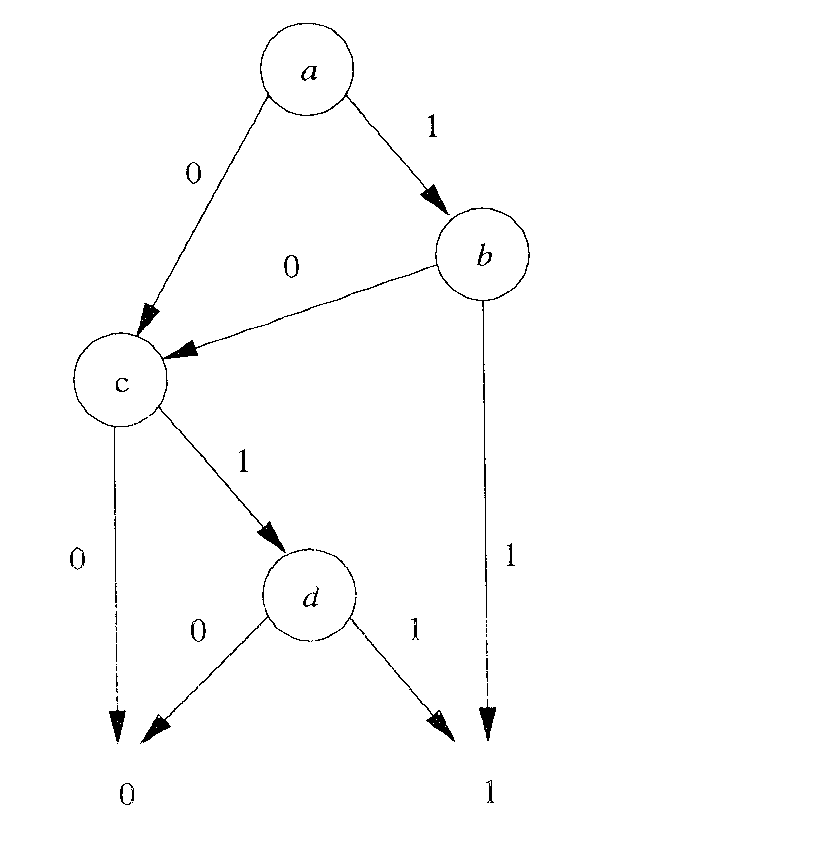
\includegraphics[scale=0.30]{Figuras/Arvore_BDD.png}
	\end{center}
    \legend{Fonte: \cite{clarke1994model}}
\end{figure}

\todo[inline]{Adicionar mais detalhes e descrever onde DDB é utilizado.}

\todo[inline]{Adicionar uma seção para definir model checking.}

%============================
%BOUNDED MODEL CHECKING
%============================
\subsection{\label{cap:bounded}\textit{Bounded Model Checking}}
Segundo \citeauthor{rocha2015verificaccao}, \textit{Bounded Model Checking} (BMC) é um tipo especial de \textit{Model Checking} que usualmente adota o método de satisfabilidade booleana, o qual tem sido introduzido como uma técnica complementar para diagrama de decisão binaria para aliviar o problema da explosão de estados, visto que a técnica de \textit{Model Checking} busca todos os estados possíveis para verificação.

\par
\textit{Bounded Model Checking} é uma técnica para a verificação de uma dada propriedade em uma determinada profundidade do sistema analisado. Logo, dado um sistema de transições M, uma propriedade $\phi$, e um limite (\textit{bound}) $k$, o BMC desenrola o sistema $k$ vezes e traduz o sistema em uma condição de verificação(CV) $\psi$ tal que $\psi$ é satisfeito se e somente se $\phi$ tem um contra-exemplo de profundidade menor ou igual a $k$ \cite{rocha2015verificaccao}.

\par
O \textit{Extended SMT-Based Bounded Model Checker} (ESBMC) é um \textit{Bounded Model Checking} baseado em satisfabilidade booleana (SAT\todo{Já tem suporte a SMT adicionar ao texto}) que permite verificação aritmética de overflow e undeflow, segurança de ponteiros, limite de array, de gerar propriedades de segurança em programas em C/C$++$. ESBMC utiliza uma versão modificada do CBMC no \textit{front-end} para analisar o código ANSI-C e para gerar as condições de verificação através de execução simbólica \cite{cordeiro2012smt,rocha2015verificaccao}.

\par
No ESBMC, o programa analisado é modelado em um sistema de transição de estados, conforme a trupla: $M=(S,R,S_{0})$, o qual é gerado um grafo de controle de fluxo (GFC), onde $S$ representa o conjunto de estados, $R$ $\subseteq$ $SxS$ representa as transições e $S \subseteq S$ representa o conjuto de estados iniciais. Um estado $s \in S$ consiste no valor do contador de programa (PC) e os valores de todas as variáveis dos programas. O estado inicial $S_{0}$ atribui o inicio do programa GFC ao PC, desta forma o ESBMC identifica as transições, conforme a formula lógica, $\gamma$=($S_{i}$,$S_{i+1}$) que captura as retrições sobre os valores correspondntes do PC e das variáveis do programa~\cite{cordeiro2012smt}.

\par
Segundo o site da ferramenta\todo{Qual site?}, a ferramenta permite ao usuário indicar propriedades adicionais\todo{Descrever quais propriedades o esbmc suporta} usando assertivas que também são verificadas. O ESBMC converte as condições usando diferentes técnicas de background\todo{apresentar exemplo} para posteriormente passar para verificador SMT. Outra vantagem é a ferramenta permitir verificação de software single-thread e multi-thread.

\todo[inline]{Descrever qual a razão da escolha para o trabalho, apresentar resultados do SV-COMP dos últimos 3 anos}

%============================
%REDES DE PETRI
%============================
\subsection{Redes de petri}

\todo[inline]{Apresentar definição formal para RP}

\todo[inline]{corrigir o texto abaixo RP não é uma ferramenta e sim um método de modelagem}

Redes de petri são utilizadas como ferramentas de modelagem gráfica com propriedades matemática. Como ferramenta gráfica são utilizadas como comunicação visual, como fluxogramas, por exemplo, e como ferramenta matemática podem configurar modelos matemáticos que regem o comportamento dos sistemas. A grade premissa desta ferramenta é descrever sistemas de processamento de informações caracterizados como concorrentes, assíncronos, distribuídos, paralelos, não deterministas e/ou estocásticos~\cite{murata1989petri}.

\par
As redes de petri são representados como grafos direcionais compostos por nós e arcos, conforme apresentado na \autoref{fig:rede_petri}. Os nós representam as transições e eventos e os arcos representam os pesos. Dentro desta representação, os arcos e eventos são componentes passivos enquanto as transições são ativos. A principal vantagem da utilização das redes de petri esta relacionado ao chamado "\textit{Token game}" que consiste no comportamento da rede de petri, em outras palavras, representa o funcionamento do sistema representado pela rede\cite{halder2006}.

\begin{figure}[htb]
	\begin{center}
    \caption{\label{fig:rede_petri}Rede de petri}
	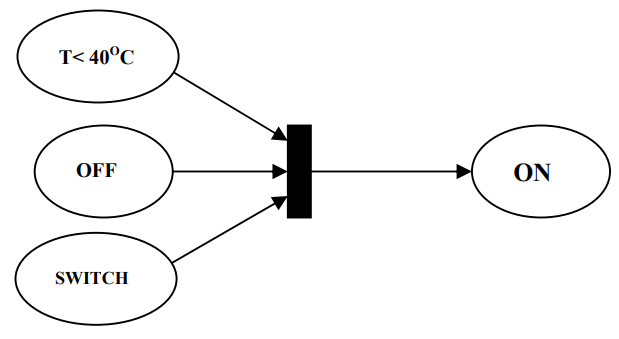
\includegraphics[scale=0.40]{Figuras/rede_petri.png}
	\end{center}
    \legend{Fonte: \cite{halder2006}}
\end{figure}

\todo[inline]{Descrever o funcionamento da RP apresentado na IMG}

\todo[inline]{Descrever quais propriedades podem ser verificadas com RP e onde será utilizado no seu trabalho.}

%============================
%VERIFICAÇÃO DE HARDWARE
%============================
\subsection{Verificação de hardware}

Para a verificação de hardware diversas técnicas têm sido propostas (\todo{Apresentar exemplos com referências}). Por meio da simulação, visa assegurar que uma implemetação, descrição do hardware em qualquer qualquer nível de abstração da hierarquia de hardware, atinja suas especificações, propriedades que devem ser respeitadas para que a corretude do mesmo seja comprovada~\cite{gupta1992formal}. A Verificação formal de hardware consiste na utilização 
% dos conceitos de verificação formal, mas também 
de técnicas para corretude de circuitos lógicos, ou seja, consiste na utilização de modelos matemáticos para descrição de propriedade e/ou de comportamento de um dado sistema~\cite{kropf2013introduction}.

\par
Entre as abordagens utilizadas na verificação formal de hardware consiste tanto na implementação quanto a especificação estarem descritas em lógica formal, neste caso a corretude será obtida através da comprovada relação entre a implementação e a especificação~\cite{seger1992introduction}. A especificação formal consiste na descrição do comportamento, bem como, das propriedades do sistema em linguagem matemática, tornando-se crucial para o processo de verificação. Na implementação formal, o nível de abstração, tais como, \textit{Gate level} e RTL são importantes informações para o desenvolvimento do formalismo, bem como as classes, por exemplo se o circuito é sequencial ou combinacional, se utiliza pipeline, etc~\cite{kropf2013introduction}.

\todo[inline]{Apresentar um exemplo de RTL}

\par
A utilização de \textit{Model Checking} também se faz presente nos modelos formais de verificação de hardware, onde apenas é utilizado o comportamento dos circuitos na verificação, de modo a verificar a se as propriedades  presentes são satisfeitas. Para isso, são utilizados os conceitos da lógica proposicional, que por meio da utilização de fórmulas que representem as propriedades dos estados, é possível realizar as verificações necessárias~\cite{seger1992introduction}.

\todo[inline]{Apresentar um exemplo com um circuito e como este pode ser verificando com model checking}
 
%============================
%VERIFICAÇÃO DE SOFTWARE
%============================
\subsection{Verificação formal de software}

% Segundo \citeauthor{rocha2015verificaccao}, o
Observa-se que o uso de verificacão de software tem sido feito aplicado em muitas áreas, tais como, infraestruturas industriais de missão critica e de segurança.  Logo, existe a necessidade de garantir a corretude destes sistemas. Devido a isso, a verificação formal tem sido utilizada em três principais abordagens, sendo elas~\cite{cousot2010gentle,d2008survey}:

\todo[inline]{Apresentar exemplos para os métodos apresentados abaixo}

\begin{itemize}
 \item \textbf{Métodos dedutivos:} Produzem provas matemáticas formais de corretude usando provadores de teoremas ou assistentes de prova para execução da prova e necessitam da interação humana para prover os argumentos~\cite{cousot2010gentle};
  \item \textbf{Verificação de modelos:} Exploram exaustivamente modelos de execuções de programa, que podem ser sujeitos a explosão combinatória, necessário a intervenção humana para geração dos modelos~\cite{rocha2015verificaccao};
  \item \textbf{Analise estática:} Engloba diversas técnicas para calcular automaticamente informações sobre o comportamento de um programa sem executá-lo, sendo utilizado em otimização de código e verificação em compiladres~\cite{d2008survey}.
\end{itemize}

Segundo \citeauthor{rocha2015verificaccao}, na verificação formal de software apresentam-se dificuldades, tais como: quais as propriedades são de interesse na verificação em tempo de execução; e impossibilidade matemática de provar a corretude de propriedades não triviais no comportamento de programas 
% , devido ao computador ser um dispositivo finito
~\cite{cousot2010gentle}. 

%============================
%LÓGICA PROPOSICIONAL
%============================
\subsection{Lógica proposicional}
A lógica proposicional é uma linguagem formal onde é definida um alfabeto e conectivos proposicionais, e um conjunto de regras gramaticais, as quais serão utilizadas para construção das proposições\cite{souza2017logica}. Porém apesar de importante, ela é limitada, não podendo expressar sentenças elementares importantes, tais como a da aritmética elementar. Por exemplo:
\begin{enumerate}
\item Todos são mortais.
\item Alguém é bondoso.
\end{enumerate}
Na lógica preposicional, não poderiam ser analisadas, pois não teria como decompor ambas em sentença e assim não teria como analisar as diferenças entre ambas\cite{abe2002introducao}. Contudo, no exemplo:
\begin{enumerate}
\item Existem cavalos com patas verdes.
\end{enumerate}
A relação criada pela frase poderia  a ser analisada pela lógica proposicional\cite{abe2002introducao}.

Segundo \citeauthor{souza2017logica}, alfabeto da lógica proposicional é formado por símbolo de pontuação, símbolos proposicionais e conectivos proposicionais, onde cada um apresenta uma função em específico, sendo:
\begin{itemize}
\item \textbf{Símbolos de pontuação: }Apenas dois símbolos de pontuação são utilizados o "(" e o ")".
\item \textbf{Símbolos proposicionais:} São utilizados para representar as proposições, onde um símbolo \textit{P} pode ser utilizado para representar uma proposição qualquer, por exemplo: \textit{P}="Está chovendo". O conjunto de símbolos proposicionais é infinito e enumerável, sendo possível representar infinitos e enumerável conjunto de proposições.
\item \textbf{Conectivos proposicionais:} São os símbolos usando frequentemente na matemática. Os símbolos recebem a seguinte denominação: 
\begin{enumerate}
\item \textbf{$\neg$}: Representa a partícula de negação, ou seja, "Não".
\item \textbf{$\lor$}: Representa a partícula "Ou"
\item \textbf{$\land$}: Representa a partícula "E"
\item \textbf{$\rightarrow$}: Representa a partícula "Se então ou implica".
\item \textbf{$\Leftrightarrow$}: Representa a partícula "Se, e somente se".
\end{enumerate} 
\end{itemize}

Ainda segundo \citeauthor{souza2017logica}, existem as fórmulas que são constituídas de forma indutiva, a partir de símbolos do alfabeto conforme as regras apresentadas abaixo:
\begin{itemize}
\item Todo o símbolo preposicional é uma fórmula
\item Se \textit{H} é uma fórmula, então ($\neg$\textit{H}), a negação de \textit{H}, é uma fórmula.
\item Se \textit{H} e \textit{G} são fórmulas, então a disjunção de \textit{H} e \textit{G}, dada por (\textit{H} $\lor$ \textit{G}), é uma fórmula.
\item Se \textit{H} e \textit{G} são fórmulas, então a conjunção de \textit{H} e \textit{G}, dada por (\textit{H} $\land$ \textit{G}), é uma fórmula.
\item Se \textit{H} e \textit{G} são fórmulas, então a implicação de \textit{H} e \textit{G}, dada por (\textit{H} $\rightarrow$ \textit{G}), é uma fórmula. Neste caso, \textit{H} é o antecedente e \textit{G} consequente da fórmula.
\item Se \textit{H} e \textit{G} são fórmulas, então a bi-implicação de \textit{H} e \textit{G}, dada por (\textit{H} $\leftrightarrow$ \textit{G}), é uma fórmula. Neste caso, \textit{H} é o lado esquerdo e \textit{G} o lado direito da fórmula.
\end{itemize}


%============================
%Property Specification Language - PSL
%============================
\subsection{Linguagem de especificação de propriedades}
Linguagem de especificação de propriedades, do inglês \textit{Property Specification Language} - PSL, é uma notação formal para especificação de comportamento em sistemas eletrônicos, compatível com as linguagens VHDL, Verilog, SystemC e SystemVerilog. Destina-se a utilização para a especificação funcional, mas também para entrada de ferramentas de verificação. A especificação do PSL é a utilização de assertivas sobre propriedades de um sistema, sendo estas propriedades constituídas de três elementos: expressões boolenas, expressões sequenciais e operadores temporais\cite{IEEEPSL}.

\par
Segundo \cite{IEEEPSL}, o PSL foi totalmente desenvolvida com o intuito fornecer leitura e escrita de fácil entendimento, sintase concisa, semântica formal e rigorosamente bem definida e ser matematicamente precisa, visto a utilização da mesma em processo de verificação. Entre os pontos principais do PSL encontram-se:
\begin{itemize}
\item Sintaxe concisa,
\item Semântica formal rigorosamente definida,
\item Permite a especificação de propriedades reais,
\end{itemize}

\par
O PSL pode ser utilizado para capturar requisitos relativos ao comportamento total do projeto, bem como, sobre o modo que o mesmo deverá operar no ambiente, ms também para capturar requisitos comportamentais e os pressupostos que surgem durante o processo de design. Ambas podem ser utilizadas para verificação de sistemas \cite{IEEEPSL}.
%============================
%Assertion-based verification - ABV
%============================
\subsection{Verificação baseada em assertivas}
Verificação baseada em assertivas, do inglês\textit{Assertion-based verification} - ABV, é um paradigma de verificação igualente adequado para verificação formal e abordagens baseadas em simulação\cite{boule2005incorporating} e em conjunto com a tecnica de PSL tem ganhado aceitação como um método essencial para verificação funcional do hardware\cite{DahanCombining}.

\par
A técnica utiliza assertivas, que são declaração adicionadas ao projeto com o intuito de especificar o comportamento do projeto, podendo escritos em PSL ou em SVA(\textit{System Verilog Assertions.}\cite{boule2005incorporating}. No caso deste projeto será utilizado a PSL, devido a mesma ser utilizada juntamente com a linguagem VHDL.

\par
Com o ABV e as assertivas, circuito pode ser verificado usando técnicas de simulação e/ou verificação, por exemplo, \textit{Model Checking}, para garantir que o mesmo esteja de acordo com o pretendido co projeto\cite{DahanCombining}. 

Na \autoref{fig:assertiva} apresenta o modelo de assertiva utilizada no projeto, utilizando de um modelo próprio para assertivas, unindo as funcionalidades já existentes nas assertivas do VHDL, mas também novas, fornecendo assim mais propriedades a serem analisadas.

\begin{figure}[thp]
\caption{\label{fig:assertiva} Exemplo de declaração de assertiva no VHDL.}
	\begin{center}
    \begin{minipage}{0.9\textwidth}
    \begin{lstlisting}       
library ieee;
use ieee.std_logic_1164.all;

entity AND_ent is
port(   x,y: in bit;
        F: out bit
);
end AND_ent;

architecture behav1 of AND_ent is
begin
	--@c2vhdl:ASSERT
    --assert not (x='0' and y='1')
    --report "Both values of signals x and y are equal to 1"
    --severity ERROR;
    --@c2vhdl:END

	process(x, y)
    	begin
        	if ((x='1') and (y='1')) then
            	F <= '1';
        	else
            	F <= '0';
        	end if;
    	end process;4
end behav1;

\end{lstlisting}
    \end{minipage}
	\end{center}
    \legend{Fonte: Própria.}
\end{figure}
%============================
%PROPRIEDADES DE SEGURANÇA
%============================
\subsection{Propriedades de segurança}
Propriedades de segurança é um meio de validação do comportamento de um determinado sistema, de modo que ser uma propriedade de segurança for violada, então através de uma execução finita, é possível verificar tal erro. Algumas propriedades de segurança, no entanto, podem impor requisitos em fragmentos de caminho finito e não podem ser verificadas considerando apenas os estados alcançáveis. \cite{baier2008principles}.

\par
Segundo \cite{clarke2003verification}, podemos definir uma propriedade de segurança como: \textit{dado um sistema de transições $ST = (S, S_0, E)$, seja um conjunto $B \subset S$ que especifica um conjunto de maus estados tais que $S_0 \cap B = \emptyset$, pode-se dizer que $ST$ é seguro com relação a $B$, denotado por $ST \models AG\neg B$ se não existe um caminho no sistema de transição do estado inicial $S_0$ até o estado $B$, de outro modo é dito que $ST$ não é seguro}.
%============================
%TECNICAS DE COMPILADORES
%============================
\section{Técnicas de compiladores}
\par
Compiladores são sistemas de software utilizados para tradução de uma linguagem de programação para outra, ou seja, o programa da linguagem fonte é lido e traduzido para um código equivalente na outra linguagem, ou linguagem alvo. Geralmente utilizada para transformar trechos de código em uma linguagem a ser executada pelo computador\cite{aho2007compilers}. 

\par
Diversas técnicas podem ser utilizadas nas diversas etapas, até que o código seja traduzido, tais como LL(1) e LR na análise sintática e \textit{Peephole} na otimização de código\cite{aho2007compilers}. Neste projeto serão focados as áreas de transformações de código e otimização de código.
%============================
%TRANSFORMAÇÕES DE CÓDIGO
%============================
\subsection{Transformações de código}
\par
Transformações de código correspondem a uma complexa função que envolve analise de fluxo de dados e modificação completa do programa e são parte integral da alta performance e sistemas computacionais. Podem ser classificados em transformações escalares que reduzem o número de instruções a serem executadas no programa ou transformações paralelas que maximizam o paralelismo.\cite{srikant2002compiler}

\par
A \autoref{fig:cod_vhdl} representa o trecho de código apresentado na \autoref{fig:assertiva}. O trecho representa o comportamento das entradas, neste caso de um código da porta AND. E a figura \autoref{fig:cod_c} representa a tradução deste trecho em código na linguagem C. Esta tradução foi realizada pela ferramenta V2C, utilizada neste projeto.

\begin{figure}[thp]
\caption{\label{fig:cod_vhdl} Trecho de código em VHDL representando porta AND.}
	\begin{center}
    \begin{minipage}{0.9\textwidth}
    \begin{lstlisting}       
	process(x, y)
    	begin
        	if ((x='1') and (y='1')) then
            	F <= '1';
        	else
            	F <= '0';
        	end if;
    	end process;
\end{lstlisting}
    \end{minipage}
	\end{center}
    \legend{Fonte: Própria.}
\end{figure}

\begin{figure}[thp]
\caption{\label{fig:cod_c} Trecho de código traduzido para linguagem C.}
	\begin{center}
    \begin{minipage}{0.9\textwidth}
    \begin{lstlisting}       
   /* Start of Translation */
   /* p0: */
   if (chg[x] || chg[y]) {
      if (((old[x]==1) && (old[y]==1))) {
      	new[f]=1;
      }
      else {
      	new[f]=0;
      }
   }
   /* End of Translation */

	\end{lstlisting}
    \end{minipage}
	\end{center}
    \legend{Fonte: Própria.}
\end{figure}
%============================
%OTIMIZAÇÃO ok
%============================
\subsection{Otimização de código}
\par
A otimização de código consiste na melhoria do código intermediário gerado pelos algoritmos de compilação com o objetivo de rodar mais rapidamente, porém outros fatores podem ser introduzidos, como algoritmos menores. Este fato não implica em afirmar que o melhor código é gerado, visto que dada a complexidade, raramente pode ser obtido que o código gerado pode ser o melhor possível\cite{aho2007compilers}.

\par
Segundo \cite{aho2007compilers}, otimização local de código consiste na otimização de um bloco básico de código, ou seja, a otimização ocorre em um trecho especifico de código. Os blocos básicos são trecho onde não ocorrem saltos ou \textit{loops}, para nenhuma outra parte do código. A otimização global de código é baseado na analise do fluxo de dados, de modo que ocorra as elminação de instruções não necessárias ou substituição mais facil. A otimização global consite na analise completa do código.

%============================
%Grafo Acliclico Direcional - GAD ok
%============================
\subsubsection{Grafo Acliclico Direcional - GAD}
\par
Grafo Aciclico Direcional é utilizado para diversos fins dentro da estrutura de compiladores, principalmente para geração da parse tree otimização de código. Pode ser usado na representação de instruções unicas blocos básicos de código\cite{aho2007compilers}. O uso de GAD permite a melhoria de de código, tais como:
\begin{itemize}
\item Elminação de subexpressões locais comuns, ou seja, expressões que o valor já foi computado anteriomente;
\item Eliminação de código morto;
\item  Reordernamento de declarações buscando reduzir o tempo que o valor temporário necessita ser preservado em um registro;
\end{itemize}

\par
\begin{figure}[thp]
\caption{\label{fig:basic_block} Exemplo de bloco basico de código.}
	\begin{center}
    \begin{minipage}{0.9\textwidth}
    \begin{lstlisting}
    a = b + c
    b = a - d
    c = b + c
    d = a - d
	\end{lstlisting}
    \end{minipage}
	\end{center}
    \legend{Fonte: \cite{aho2007compilers}}
\end{figure}

\begin{figure}[htb]
	\begin{center}
    \caption{\label{fig:gda}GAD do bloco básico da \autoref{fig:basic_block}}
	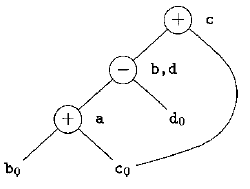
\includegraphics[scale=0.40]{Figuras/GDA.png}
	\end{center}
    \legend{Fonte: \cite{aho2007compilers}}
\end{figure}

Na \autoref{fig:basic_block} apresenta um bloco básico com algumas instruções, no caso aresentando 4 operações entre somas e multiplicação e a partir deste bloco a \autoref{fig:gda} apresenta o GDA deste trecho de código. Nele aprsenta cada nó como uma operação especifica e os terminais como as parcelas das operações.

%============================
%Grafo de Fluxo de Controle - GFC 
%============================
\subsubsection{Grafo de Fluxo de Controle - GFC}
\par
Grafo de fluxo de controle corresponde a um grafo direcionado, no qual cada nó representa blocos básicos e cada aresta representa os caminhos de fluxo entre os blocos basicos.\cite{allen1970control}. É importante ressaltar que saltos determinam o final de um determinado bloco básico, ou seja, saltos indicam um caminho para uma nova região de código básico.\cite{aho2007compilers}.


%============================
%Eliminção de código morto 
%============================
\subsubsection{Eliminção de código morto}
\par
Elimincação de código morto é uma técnica busca a eficiência de um programa evitando a execução de instruções não necessária no tempo de execução.\cite{knoop1994partial}. Código morto consiste em instruções que não serão alcançáveis durante o fluxo do programa, sendo esta técnica basicamente a a retirada de qualquer variável que não será utilizada em qualquer outro nó do grafo\cite{aho2007compilers}.

\par
A utilização de GAD corresponde na eliminação de qualquer nó raiz, ou seja, nó sem ancestrais, as quais não esteja ativa anexada a mesma. A execução repetida desta operação removerá todos os nós correspondentes a código morto\cite{aho2007compilers}.

\begin{figure}[htb]
	\begin{center}
    \caption{\label{fig:elimicacao_codigo}GAD do bloco básico da \autoref{fig:basic_block}}
	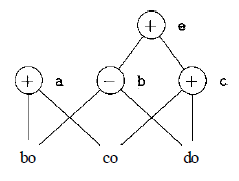
\includegraphics[scale=0.70]{Figuras/eliminacao_codigo.png}
	\end{center}
    \legend{Fonte: \cite{aho2007compilers}}
\end{figure}

Na \autoref{fig:elimicacao_codigo}, supondo que os nós a,b e c estejam ativa, porém o nó é não esteja, o ultimo pode ser eliminado imediatamente. Os nós restantes continuam no GDA, a menos que não tenho variáveis ativas atreladas aos nós\cite{aho2007compilers}.
%============================
%Analise do fluxo de dados ok
%============================
\subsubsection{Analise do fluxo de dados}
\par
Analise de fluxo de dados refere-se ao conjunto de tecnicas que derivam informaçoes sobre o fluxo de dados ao longo dos caminhos de execução do programa. Para analise do programa, é necessário considerar todas as posiveis execuções através do grafo de fluxo.\cite{aho2007compilers}.

%============================
%Gerador de código ok
%============================
\subsubsection{Gerador de código}
\par
O gerador de código é responsavél pela tradução final do programa-fonte para o programa-alvo, o mesmo recebe como entrada um código intermediário juntamente com a tabela de símbolos.Faz-se necessário que o programa-fonte tenha sido analisado sintatica e lexicamente, assim evitando que erros possam ser passados para o programa-alvo, por outro lado a existencia de uma nível de otimização, faz-se opicional neste caso\cite{aho2007compilers}.

\par
O gerador de código possui três tarefs primarias, sendo as mesmas seleção de instrução, alocação de registros e atribuições. A seleção de instruções envolve a escolha das instruções apropriadas da máquina-alvo para implementar as declarações do código intermediario. A atribuição e atribuição de registros envolve a decisão sobre os valores a serem registrados nos registros\cite{aho2007compilers}.

%------------------------------------------------------------
% Revisão de Literatura
%------------------------------------------------------------
\chapter{TRABALHOS CORRELATOS}
\label{chapter:correlatos}

\todo[inline]{Sugiro apenas mencionar que foi feito a revisão sistemática; o que já foi feito e os resultados. As outras seções sobre RS e mover para apêndice.}

%==========================================================
% REVISÃO SISTEMÁTICA
%==========================================================
\section{Revisão sistemática}

A revisão sistemática consiste é um método de identificação, análise e interpretação de pesquisas relevantes em determinada área ou questão de pesquisa. Para execução da revisão sistemática se requer um esforço maior, em comparação as pesquisas tradicionais, sendo necessário seguir uma sequência de passos metodológicos sobre a área ou questão de pesquisa ao qual deseja ser feita a pesquisa~\cite{kitchenham2004procedures}.

Para a execução da revisão sistemática, é necessário um esforço considerável, se comparado a uma revisão informal a literatura. Enquanto que a revisão de literatura informal é conduzida de forma \textit{ad-hoc}, sem planejamento e critérios de seleção estabelecidos a priori, a revisão sistemática requer um protocolo formal bem definido, com uma sequência de passos metodológicos, para conduzir uma pesquisa sobre o tema ao qual deseja-se realizar a pesquisa~\cite{MafraTravassos}.

A aplicação da revisão sistemática requer que seja seguido um conjunto bem definido e sequêncial de passos, seguindo um protocolo de pesquisa desenvolvido previamente. Através deste método é possível realizar uma extensa pesquisa, contemplando uma grande quantidade de informações sobre o assunto pesquisado~\cite{MafraTravassos}. Este protocolo é construído considerando um tema específico que representa o elemento central da investigação, onde os passos da pesquisa, as estratégias definidas para coletar as evidências e o foco das questões de pesquisa são definidas explicitamente, de tal forma que outros pesquisadores sejam capazes de reproduzir o mesmo protocolo de pesquisa~\cite{biolchini2005systematic}.

Segundo \citeauthor{MafraTravassos}, o processo para a condução de revisões sistemáticas envolve três etapas:
\begin{enumerate}
  \item \textbf{Planejamento da Revisão:} os objetivos da pesquisa são listados e o protocolo da revisão é definido.
  \item \textbf{Condução da Revisão:}nesta atividade, as fontes para a revisão sistemática são selecionadas, os estudos primários são identificados, selecionados e avaliados de acordo com os critérios de inclusão, exclusão, e de qualidade estabelecidos durante o protocolo da revisão.
  \item \textbf{Análise dos Resultados:} os dados dos estudos são extraídos e sintetizados para análise e apresentação dos resultados.
\end{enumerate}

Vale ressaltar que como o objetivo deste trabalho é realizar um estudo exploratório de caracterização de área podemos dizer que esta revisão sistemática se caracteriza como uma quasi-sistemática~\cite{travassos2008environment}, pois segue o mesmo processo da revisão sistemática e preserva o rigor e mesmo formalismo para as fases metodológicas de elaboração de protocolo e execução da revisão, mas sem a aplicação de uma meta-análise a princípio, que pode ser aplicada posteriormente.

%==========================================================
%PLANEJAMENTO DA REVISÃO SISTEMÁTICA
%==========================================================
\subsection{Planejamento da Revisão Sistemática}

\textbf{Objetivo:} Este estudo tem o objetivo esquematizado a partir da estrutura do paradigma GQM (do ingles \textit{Goal,Question and Metric})\cite{basili1994experience}.

\begin{table}[h!]
\centering
\label{}
\begin{tabularx}{\textwidth}{|l|X|}
\hline
Analisar & Publicações científicas através de um estudo baseado em revisão sistemática \\ \hline
Com propósito de & Identifica-las \\ \hline
Com relação as & Vantagens e desvantagens da utilização de assertiva e transformações de código na verificação do código na linguagem de descrição VHDL \\ \hline
Do ponto de vista do & Pesquisador \\ \hline
No contexto & Acadêmico ou industrial para verificação de assertivas na linguagem de descrição VHDL \\ \hline
\end{tabularx}
\caption{Objetivo do estudo utilizando o paradigma GQM}
\end{table}

\textbf{Formulação da Pergunta:} Buscamos respostas para as seguintes perguntas:
\begin{itemize}
\item \textbf{Q1:} Quais são os métodos para verificação de circuitos lógicos descritos na linguagem de programação VHDL?
	\begin{itemize}
	\item \textbf{Q1.1:} Foi desenvolvido e está disponível alguma ferramenta para aplicação do método?
	\item \textbf{Q1.2:} Qual a técnica de exploração de estados para circuitos lógicos?
	\item \textbf{Q1.3:} O método proposto é baseado em técnicas de verificação de software?
	\item \textbf{Q1.4:} Como o método proposto valida pré e pós condições no programa?
	\item \textbf{Q1.3:} Foi utilizado algum \textit{benchmark} de programas em VHDL para experimentação e o mesmo encontra-se disponível?
	\item \textbf{Q1.4:} Quais as perspectivas futuras para melhorar da aplicação do método proposto?
	\end{itemize}
\end{itemize}

\textbf{Escopo da pesquisa:}Na delimitação do escopo da pesquisa foram estabelecidos critérios, buscando garantir a viabilidade da execução, acessibilidade dos dados e abrangência do estudo realizado. A pesquisa dar-se-á a partir de bibliotecas digitais através das suas respectivas máquinas de busca e, quando os dados não estiverem disponíveis eletronicamente, através de consultas manuais.

\textbf{Critérios de Seleção de Fontes.} Para as bibliotecas digitais é desejado:
\begin{itemize}
  \item Possuir uma máquina de busca que permita o uso de expressões lógicas ou mecanismo equivalente.
  \item Incluir em sua base, publicações de exatas ou correlatas que possuam relação direta com o tema a ser pesquisado
  \item As máquinas de busca deverão permitir a busca no texto completo das publicações.
\end{itemize}

Segundo \citeauthor{rocha2015verificaccao}, os mecanismos de busca utilizados devem garantir resultados únicos através da busca de um mesmo conjunto de palavras-chaves (\textit{string} de busca). Quando isto não for possível, deve-se estudar e documentar uma forma de minimizar os potenciais efeitos colaterais desta limitação.

\textbf{Métodos de Busca das Publicações.} As fontes digitais foram acessadas via Web, através de expressões de busca pré-estabelecidas. A biblioteca digital consultada foi a Scopus, acessível em http://www.scopus.com. Segundo a editora \citeauthor{Elsevier}, a Scopus é uma das maiores bases de dados de resumos e citações da literatura de pesquisa \textit{peer-reviewed} com mais de $22,800$ títulos de mais de $5,000$ editoras internacionais abrangendo as áreas de tecnologia, medicina, artes, ciências sócias e com atualizações diárias. Entre as editoras podemos citar: Springer \cite{Springer}; IEEE Xplore Digital Library \cite{IEEE};ACM Digital Library \cite{ACM} ; ScienceDirect/Elsevier \cite{B.V}; Wiley Online Library \cite{Sons}; dentre outras.

\textbf{\textit{String} de Busca.} A \textit{string} de busca foi definida segundo o padrão PICO (do inglês \textit{Population, Intervention, Comparison, Outcomes}) \cite{kitchenham2009systematic}, conforme a estrutura abaixo:
\begin{itemize}
	\item População: Trabalhos publicados em conferências e periódicos que relacionam verificação de propriedades de circuitos lógicos em códigos para a descrição de hardware.

	\item Intervenção: Verificação de propriedades relacionadas a verificação de circuitos para as diferentes estruturas das linguagens de descrição de hardware;

	\item Comparação: análise de cobertura e suporte das abordagens identificadas para a verificação de propriedades das linguagens de descrição de hardware;

	\item Resultados: a partir da descrição das abordagens pretende-se verificar a cobertura que cada abordagem apresenta na manipulação das diferentes estruturas da linguagem de descrição de hardware para a verificação de propriedades baseada em assertivas.
\end{itemize}

Segundo \citeauthor{rocha2015verificaccao}, como este estudo representa um estudo de mapeamento/caracterização, a string de busca foi definida de acordo com dois aspectos: População e Intervenção, como é apresentado na estrutura abaixo. Posteriormente esta mesma \textit{string} de busca será executada na biblioteca Scopus para busca de artigos e publicações de modo a gerar uma interseção entre população e intervenção.
\begin{itemize}
\item População: publicações que fazem referência a verificação de propriedades de circuitos lógicos e sinônimos:
	\begin{itemize}
	\item \textbf{Palavras-chaves:} "circuit checker" OR "circuit verification" OR "contract based verification" OR "code analysis" OR "static analysis" OR "dynamic analysis" OR "safety verification" OR "RTL analysis" OR "program analysis" OR "property verification" OR "formal verification" OR "model checking" OR "model checker" OR "hardware checker" OR "hardware verification" OR "validity checker" OR "hardware assertion" OR "assertion checker" OR "assert verification" OR "assertion-based verification" OR "assertion based verification" OR "assertion-based design" OR "bit level verification"
	\end{itemize}
\item Intervenção: Verificação de circuitos e sinônimos:
	\begin{itemize}
	\item \textbf{Palavras-chaves:}"hardware statement" OR "hardware code" OR "hardware source code" OR "hardware semantics" OR "hardware property" OR "logical gates" OR "sequential circuit" OR "parallel circuit" OR "real circuits" OR "complex circuits" OR "control circuitry" OR ”software netlist” OR “hardware emulation” OR “silicon debug”
	\end{itemize}
\end{itemize}


%==========================================================
%PROCEDIMENTOS DE SELEÇÃO E CRITERIOS
%==========================================================
\subsubsection{Procedimentos de Seleção e Critérios}

A estratégia de busca será aplicada por um pesquisador para identificar as publicações em potencial. A seleção das publicações dar-se-á em 2 etapas, conforme apresentado a seguir.

% porém o terceiro filtro não foi executado nesta etapa do projeto, resumindo-se em apenas 3 etapas:
\begin{enumerate}
\item \textbf{Seleção e catalogação preliminar dos dados coletados:} A seleção preliminar das publicações será feita a partir da aplicação da string de busca na biblioteca Scopus, o resultado desta busca corresponde a seleção preliminar. Todas as publicações serão armazenadas para análise posterior;

\item \textbf{Seleção dos dados relevantes - [1 filtro]:} A seleção preliminar com o uso da expressão de busca não garante que todo o material coletado seja útil no contexto da pesquisa, pois a aplicação das expressões de busca é restrita ao aspecto sintático. Por isso, é necessário a criação de filtros de exclusão e inclusão, de modo a classificar os artigos e publicações que se enquadram no contexto da pesquisa realizada. Nesta epata apenas serão lidos o título, abstracts, e palavras-chaves e classificar de acordo com os filtros, ou seja, se será aceito ou excluído. Devem ser excluídas as publicações contidas no conjunto preliminar que:
	\begin{itemize}
	\item \textbf{CE1-01:} Não serão selecionadas publicações em que as palavras-chave da busca não apareçam no título, resumo e/ou texto da publicação (excluem-se os seguintes campos: as seções de agradecimentos, biografia dos autores, referências bibliográficas e anexas).
	\item \textbf{CE1-02:} Não serão selecionadas publicações em que descrevam e/ou apresentam ‘keynote speeches’, tutoriais, cursos e similares.
	\item \textbf{CE1-03:} Não serão selecionadas publicações em que o contexto das palavras-chave utilizadas no artigo leve a crer que a publicação não cita uma abordagem para verificação/validação de códigos para descrição de hardware.   
	\item \textbf{CE1-04:} Não serão selecionadas publicações em que o contexto das palavras-chave utilizadas no artigo leve a crer que a publicação não cita uma abordagem para verificação de código de descrição de hardware baseado em assertivas ou propriedades de verificação de hardware.
\end{itemize}

Podem ser incluídas apenas as publicações contidas no conjunto preliminar que:

	\begin{itemize}
	\item \textbf{CI1-01:}Podem ser selecionadas publicações em que o contexto das palavras-chave utilizadas no artigo leve a crer que a publicação cita uma abordagem para verificação de código de descrição de hardware baseado em assertivas ou propriedades de verificação de hardware.
	\item \textbf{CI1-02:}Podem ser selecionadas publicações em que o contexto das palavras-chave utilizadas no artigo leve a crer que a publicação cita recomendações de melhoria na utilização de abordagens para verificação de código de descrição de hardware baseado em assertivas ou propriedades de verificação de hardware.
	\end{itemize}
	
%=======================
%Filtro 2
%=======================
\item \textbf{Seleção dos dados relevantes - [2 filtro]:} Apesar do 1º filtro limitar o universo de busca, infelizmente não há garantias de que todo material selecionado no filtro anterior seja útil no contexto da pesquisa. Neste caso, novos filtros são gerados, buscando, da mesma forma que o primeiro filtro, classificar os artigos e publicações que se enquadram no contexto da pesquisa. Para este filtro é necessário a leitura na integras dos artigos selecionados anteriormente. O objetivo é identificar que relacionam assertivas e/ou propriedade de verificação de hardware.
    \begin{itemize}
    \item \textbf{CS2 -ASS -VER\_HARD:} Não devem ser selecionadas publicações que não contextualizem verificação de hardware e não citam assertivas
    \item \textbf{CS2 +ASS -VER\_HARD:} Não devem ser selecionadas publicações que não contextualizem verificação de hardware, mas citam assertivas
    \item \textbf{CS2 -ASS +VER\_HARD:} Não devem ser selecionadas publicações que contextualizam verificação de hardware, mas citam assertivas.
    \end{itemize}
Dessa forma, todas as publicações devem respeitar o critério abaixo:
	\begin{itemize}
	\item \textbf{CS3 +ASS +VER\_HARD:} Serão selecionadas publicações que contextualizam verificação de hardware e citam assertivas em seu contexto.
	\end{itemize}     	
\end{enumerate}

\par
Devido ao tempo necessário para o desenvolvimento execução dos filtros da revisão sistemática serem extensos, apenas o primeiro filtro foi executado neste projeto, mesmo que os parâmetros para o segundo filtro já tenho sido desenvolvidos. Em contra partida foram selecionados $6$ artigos que serviram como ferramentas de estudo para o desenvolvimento da metodologia que será apesentada no~\autoref{chapter:metodo}.

%====================================
%REVISÃO DA LITERATURA
%====================================
\section{Revisão da literatura}
Nesta sessão serão apresentados trabalho relevantes para o desenvolvimento do método proposto que foram identificados utlizando a revisão sistemática mencionado anteriormente. Os artigos apresentam técnicas de transformações de código, utilização de \textit{Assertion-Based Verification} e PSL para verificação de hardware.

\subsection{V2c-A verilog to C translator}

O artigo de \citeauthor{mukherjee2016v2c} apresenta uma ferramenta implementada em C++ chamada \texttt{v2c} para transformação de código da linguagem de descrição Verilog para linguagem de programação C. A ferramenta é executada a nível de palavra, visto que esta abordagem garante uma aumento na escalabilidade, mas também proporionando que técnicas, como interpolação\todo{adicionar referência} e aceleração de loop\todo{adicionar referência} possam ser utilizadas para verificação, algo inviavél, caso a tradução fosse executada a nível de bit. O sistema recebe como entrada um código em Verilg, onde são aplicadas regras semânticas e mapeando os bit de operação, chamado software \textit{netlist}. Após isso, o código intermediário é convertido para C.

\par
A contribuição deste trabalho\todo{Qual trabalho?} consiste na utilização de transformações de código como base principal e partindo deste pressuposto torna-se vantajoso devido a utilização de outras ferramentas que não apresente suporte a certas linguagens, tais com a ferramenta ESBMC, utilizada neste trabalho, não apresenta suporte a VHDL, porém apresenta suporte as linguagens C/C++. Em outras palavras, a contribuição deste trabalho\todo{Qual trabalho?} foi a utilização de traduções de códigos e utilizado este conceito como modelo de entrada para analise de circuitos.

% ====================================================
\subsection{Unbounded safety verification for hardware using software analyzers}
% ====================================================

No artigo de \citeauthor{mukherjee2016unbounded} foi apresentado uma metodologia que aborda a utilização de técnicas e analisadores de software, com o objetivo de 
% utiliação analises de hardware e software para
de abordar a análise de circuitos e com isso trançar um paralelo entre as abordagens. Para testes foram utilizadas três metodologias de análise, usando interpolação\todo{adicionar referência}, \textit{k-induction}\todo{adicionar referência} e tecnologias hibrídas. Como resultante dos testes, foi observado as principais causas de erros, por exemplo, bits não preciso e no caso das operações a \textit{bit-level} ocorria perda de informações. Também foi obeservado que apesar de não serem otimizadas para análises de hardware, alguns analisadores de softaware podem, dependendo da técnica utilizada no analisador, ser utilizada para analise de hardware\todo{Descrever qual o motivo.}.

\par
% No artigo foi apresentado um metodologia essencial para o desenvolvimento deste projeto, visto que 
A utilização de técnicas de análise de software para o desenvolvimento de análise de \textit{hardware} é o foco a ser abordado neste neste trabalho de maneira prática, utilizando os princípio analisados por \cite{mukherjee2016unbounded}. Neste contexto, o objetivo deste trabalho é a utilização de técnicas de software para análise de circuitos, diferente do artigo apresentado acima que busca utilização uma abordagem mais complexa provando a possibilidade da utilização de técnicas de analise de software no contexto da verificação de hardware.

\todo[inline]{A última frase está confusa, no meu entedimento é o mesmo sentido.}

% ====================================================
\subsection{Formal verification of timed VHDL programs}
% ====================================================

No trabalho apresentado por \citeauthor{bara2010formal} é proposto uma abordagem para a análise de tempo relacionado a cada porta lógica dentro de um dado circuito analisado. A abordagem apresenta a tradução de um circuito lógico codificado em VHDL para um formalismo baseado em automato de tempo\todo{referência}. Tal formalismo é representado por uma automato de estados finitos com relogios simbólicos que evoluem em taxa uniforme. A tradução é executada de modo automatico, baseado na emulação da propagação de cada transação ao longo de cada sinal, o seja, são automatos programados e cronometrados do circuito. Após a tradução para automato, a analise é feita pela ferramenta UPPAL\todo{referência} que é um \textit{model checking} de verificação de propriedades de tempo. Seguindo esta metodologia a análise pode ser extraida de modo independente de cada bloco, desta forma a análise é feita de forma mais precisa, podendo ser analisado inumeros fatores, tais como limites de intervalo e sinal de correlação.

\par
O artigo apresenta uma abordagem de tempo, que torna-se interessante adição ao método. Porém até o momento a função não foi implementada ficando a trabalho futuros.
\todo[inline]{Expandir o texto acima, exemplo, descrever como o método poderia ser incluindo no seu TCC.}

% ====================================================
\subsection{On the use of assertions for embedded-software dynamic verification}
% ====================================================

Em \citeauthor{di2012use} é apresentado uma metodologia para a integração dinamica de \textit{Assertion-Based Verification} para várias fases da análise da verificação de fluxo em sistemas embarcados, por exemplo, emulação, diagnosticos e \textit{Debug}, mas também um ferramenta chamada \textit{RadCheck}. O metodo de aplicação, chamado \textit{V-model} é dividido em fases de verificação em paralelo com as fases de \textit{design} do circuito. Com base no \textit{V-model}, o método é aplicado, iniciando com o nível de sistema e as especificação do sistema, neste caso especificado usando PSL. Neste nível é especificado todas as funcionalidades gerais da aplicação. No nível de integração visa investigar problemas de interação que possam ocorrer, definindo propriedades que cobrem incrementalmente as unidades estruturais interativas de aplicação. No nível de unidade descrevem comportamentos internos e são definidas através de parâmetros de entrada/saída das unidade e estruturas de dados internas.

\par
A contribuição deste projeto está relacionado a utilização de assertivas no contexto da verificação de software. As assertivas são o principal meio de análise proposto neste projeto, visto que estas mesma assertivas serão analisadas pelo ESBMC. Aliado a isso em \citeauthor{di2012use} é apresentado modelos de utilização de assertivas no processo de verificação de hardware, e tais assertivas foram adaptadas para um modelo proposto neste trabalho.

% ====================================================
\subsection{Incorporating efficient assertion checkers into hardware emulation}
% ====================================================

% \todo[inline]{Este foi o artigo que menos entendi, então tive uma pequena dificuldade para a escrita deste capitulo.}
No trabalho de \citeauthor{boule2005incorporating} é apresentado uma ferramenta de geração de assertivas no contexto da emulação de circuitos, de modo que estas assertivas descrita em PSL possam transformadas para o modelo de linguagem de descrição de hardware. Inicialmente é realizada toda análise de cada assertiva e a mesma é traduzida em partes, levando em consideração os operadores e cada estrutura, por exemplo \texttt{if-else}, utilizado na declaração da assertiva.

\todo[inline]{Apresentar um exemplo para explicar o texto acima}

\par
trabalho de \citeauthor{boule2005incorporating} consolida e apresenta aspectos importantes, tais como a utilização de uma ferramenta para geração de assertivas, o que torna-se no contexto deste projeto, extremamente importante, visto que o modelo adotado atualmente consiste tanto na geração automática das assertivas, bem como a inserção manual por parte do usuário.
%------------------------------------------------------------
% Detalhes de Desenvolvimento do Projeto
%------------------------------------------------------------
\chapter{MÉTODO PROPOSTO}
\label{chapter:metodo}
\par
Neste capítulo descreve o método proposto utilizado no desenvolvimento deste projeto. Inicialmente será apresentado o modelo geral e posteriormente as duas abordagens utilizadas com base neste método, além dos pontos principais de cada uma delas. Ambos os métodos são baseados em transformações de códigos para análise de circuitos lógicos descritos em VHDL utilizando 
\textit{Bounded Model Checking}, neste caso o \textit{model checker} ESBMC.

%======================
%Visão geral do método
%======================
\section{Visão geral}

\par
O método proposto consiste na análise de códigos VHDL através da inserção de assertivas ao código, de modo a validar ou mesmo gerar a ocorrência de erros que possam ocorrer durante a execução. Aliado a inserção de assertivas, também é utilizado a técnica de transformação de código, convertendo o mesmo de VHDL para linguagem C. 

\begin{figure}[H]
	\begin{center}
    \caption{\label{fig:metodo} Fluxograma do método proposto.}
	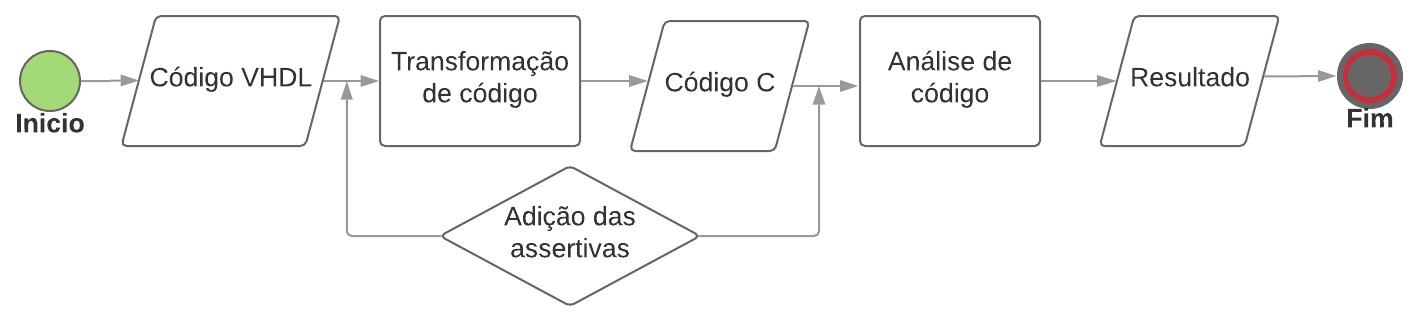
\includegraphics[scale=0.32]{Figuras/Fluxo_metodo.png}
	\end{center}
    \legend{Fonte:Própria}
\end{figure}

\par
Partindo do citado anteriormente e conforme mostrado na \autoref{fig:metodo}, o método se inicia com o código em VHDL a ser analisado. Nenhuma analise é realizada diretamente sobre o código VHDL, sendo apenas sobre o código já convertido para linguagem C, devido a existência de vários analisadores de código que são utilizados para identificação de erros nesta linguagem, por exemplo, a ferramenta ESBMC. 

\par
As assertivas podem ser inseridas antes ou depois da transformação de código. Independente do caso adotado, a mesma devem seguir o padrão aceito pela ferramenta de analise utilizada, caso contrário, a mesma não apresentará a eficácia necessária. A escolha do momento de inserção das assertivas depende principalmente do modo como a tradução ta sendo realizada e as capacidades da ferramenta de tradução em converter estas assertivas.

\par
Sendo as assertivas inseridas antes da transformação, mesma deve ser traduzida para linguagem C, seja pela ferramenta, na forma de comentário ou por meio de alguma instrumentação que venha a ser realizada no código. Esta instrumentação não deve alterar a lógica do código, pois desta forma a mesma alteraria o código que pretende ser analisado. Caso seja feita após a tradução, a mesma já pode ser inserida ao código diretamente em linguagem C.

\par
O analisador deve ser capaz de interpretar as assertivas adicionadas ao código, deste modo, um padrão deve ser implementado de acordo com as particularidades da ferramenta, neste caso, de acordo com as funções da ferramenta de análise. Deste modo, evita que erros possam ocorrer durante a análise do código.
%++++++++++++++++++++++++++++++++++++++++++++++++++++++++++
%==========================================================
%APRESENTAÇÃO DAS ABORDAGENS
%==========================================================
%++++++++++++++++++++++++++++++++++++++++++++++++++++++++++
\section{Abordagens desenvolvidas}
%\par
%Inicialmente será apresentado o método de transformação direta e todas as suas etapas e posteriormente será a presentado o método de múltiplas transformações. Com o intuito de auxiliar nas explicações apresentadas nas próximas seções, o código na \autoref{fig:code_exemplo} será utilizado nas explanações, bem como será apresentado todas as alterações do mesmo, conforme cada etapa do método. 

%\todo[inline]{Adicionar explicação que séra apresentado apenas os modelos de tradução e que a analise de código será a mesma utilizada nos dois métodos}

\par
Inicialmente será apresentado dois métodos de tradução que foram desenvolvidos durante a elaboração do trabalho. Ambos os métodos foram baseados na estrutura geral do método, utilizando o sistema de assertivas, ferramentas de transformação. Para o total funcionamento das abordagens, são realizadas instrumentações para adaptação do códigos com as ferramentas e também na execucão das mesmas. 

\par
O primeiro método chamado de transformação direta apresenta uma unica ferramenta que realizada a conversão de VHDL para C. O circuito lógico descrito em VHDL, onde as assertivas serão inseridas pelo próprio usuário do método. O código VHDL é traduzido para linguagem C e recebe uma instrumentação de código para a posterior validação do mesmo. O Código em C automaticamente gerado será processado e analisado, e de acordo com as assertivas inseridas, apresentará falha, caso alguma delas seja violada. 

\par
O segundo método chamado de multiplas trasnformações apresenta duas ferramentas de transformação, sendo a primeira de VHDL para Verilog e seguido de uma ferramenta de Verilog para C. Inicialmente o código em VHDL é passado para ferramenta juntamente com outro arquivo contendo as variáveis de entrada, saída, pré-condições e pós-condições. Seguidamente é passado para duas ferramenta de tradução e também duas etapas de instrumentação. Após as traduções, as pré-condições e pós-condições, conforme o arquivo, são adicionadas ao códigos C e o mesmo é analisado. Caso alguma condição seja violada, o contra exemplo é apresentado ao usuário.

\par
A parte referênte a analise do código será apresentada em uma única sessão, visto que ambas as abordagens apresenta a mesma ferramenta para analise e estruturas. Será demonstrado de que forma a ferramenta foi utilizada para verificação da corretude do código, através das assertivas. 

\par
O código é um conceito básico de ula, formado apenas pelas portas AND e OR, além de um inversor o qual inverte o sinal de entrada, caso seja necessário. A saída deste inversor é ligada as portas AND e OR, e a saída desta porta é ligada a um multiplexador de duas entradas. Ao final, a saída do multiplexador será um dos sinais de entrada, ou seja, ou o sinal enviado pela porta AND ou pela porta OR e este sinal de saída será determinado de acordo com o sinal de escolha enviado ao multiplexador.

\begin{figure}[H]
\caption{\label{fig:code_exemplo} Exemplo de código VHDL de ULA com portas AND e OR.}
	\begin{center}
    \begin{minipage}{0.7\textwidth}
    \begin{lstlisting}       
library ieee;
use ieee.std_logic_1164.all;

ENTITY Ula_tcc IS
PORT(A,B,Binvertido,Op1:IN std_logic;
	  Resultado:OUT std_logic);
END Ula_tcc;

ARCHITECTURE Ula_tcc_behavl OF Ula_tcc IS
SIGNAL and_port: std_logic;
SIGNAL or_port: std_logic;
SIGNAL mux2x1: std_logic;
BEGIN
	PROCESS(A,B,Binvertido,Op1)
	BEGIN
		IF(Binvertido = '0') THEN
			mux2x1 <= B;
		ELSE
			mux2x1 <= NOT B;
		END IF;
		and_port <= A AND mux2x1;
		or_port <= A OR mux2x1;
		IF(Op1 = '0') THEN
			Resultado <= and_port;
		ELSIF(Op1 = '1') THEN
			Resultado <= or_port;
		END IF;
	END PROCESS;
END Ula_tcc_behavl;
    \end{lstlisting}
    \end{minipage}
	\end{center}
    \legend{Fonte: Própria.}
\end{figure}

\subsection{Método de transformação direta}
%==========================================================
%Visão geral do método de transformação direta
%==========================================================
%\subsection{Visão geral do método de transformação direta}
%\par
%O método proposto consiste inicialmente em receber como entrada um circuito lógico descrito em VHDL, onde uma dada propriedade representada em uma assertiva será analisada, as assertivas serão inseridas de automaticamente pelo método ou pelo próprio usuário do método. O código VHDL analisado posteriomente é traduzido para linguagem C e recebe uma instrumentação de código (com funções especificas suportadas pelo método) para a posterior validação do mesmo. O Código em C automaticamente gerado, já instrumentado, será processado e analisado pelo ESBMC de acordo com as assertivas inseridas e ao final é apresentado o resultado. Caso alguma das assertivas seja violada, um contra-exemplo é apresentado ao usuário.

\subsubsection{Preprocessamento do VHDL e inserção de assertivas}

\par
A fase inicial do método consiste na adição das assertivas ao código VHDL. Vale ressaltar que mesmo a linguagem VHDL tendo um modelo de assertivas, tornou-se necessário a criação de um modelo próprio, baseado em comentários, para que as funções do model checker adotado fossem suportadas, como a geração de valores não determinísticos.\todo{Adicionar significado do termo} 

\par
As assertivas são adicionadas entre as tags \texttt{@c2vhdl:ASSERT} e \texttt{@c2vhdl:END} e todo trecho de código entre estas tags deve estar comentado, desta forma não apresentará erro na tradução do código em linguagem C, bem como na sintetização do código VHDL. Nas assertivas são incluídas as funções necessárias para a análise utilizando a ferramenta ESBMC. A assertiva apresenta três informações principais, sendo elas: condição, mensagem e gravidade. 

\begin{figure}[H]
\caption{\label{fig:assertiva} Exemplo de assertiva para verificação de porta \texttt{AND}.}
	\begin{center}
    \begin{minipage}{0.99\textwidth}
    \begin{lstlisting}       
--@c2vhdl:ASSERT
--assert (Resultado = '1')
--report "O resutado foi diferente a 0"
--severity ERROR;
--@c2vhdl:END
    \end{lstlisting}
    \end{minipage}
	\end{center}
    \legend{Fonte: Própria.}
\end{figure}

\par
A condição, \textbf{linha $2$} da \autoref{fig:assertiva}, representa a assertiva propriamente dita e que será analisado pela aplicação. A condição será precedida de \texttt{$--$assert} e seguido ou não da palavra \texttt{not}, com isso a assertiva pode assumir valor negativo, conforme necessidade do usuário. Na \autoref{fig:assertiva} a assertiva busca verificar se a variável \texttt{Resultado} terá valor igual a $1$, com isso ao comparar o valor buscado pela assertiva e o gerado no final do código, caso ambos sejam iguais, ocorre falha na verificação. 

\par
A mensagem, \textbf{linha $3$} da \autoref{fig:assertiva}, é definida pelo usuário e será exibida caso a assertiva apresente falha, assim a mensagem pode ser utilizada como um meio de depuração das propriedades validadas. A severidade, \textbf{linha $2$} da \autoref{fig:assertiva}, pode ser definida como \texttt{error}, que representa um erro fatal e parada da verificação. A severidade do tipo \texttt{warning} que representa um erro não fatal, contabiliza as falhas das assertivas, porém não causa a parada da verificação.

\par
Juntamente com as assertivas outra função que pode ser utilizada é a função \texttt{\_\_ESBMC\allowbreak{}\_assume()} suportada pelo model checker ESBMC. Esta função utilizada em conjunto com a ferramenta ESBMC permite que durante a verificação uma variável possa ter um valor definido durante o tempo de execução da verificação. A importância desta função é fazer verificações onde se conhece os valores de entrada juntamente com o valor resultante, por exemplo, na verificação de portas lógicas.

\begin{figure}[H]
\caption{\label{fig:assertiva_assume} Exemplo de utilização da função \texttt{\_\_ESBMC\_assume()}.}
	\begin{center}
    \begin{minipage}{0.99\textwidth}
    \begin{lstlisting}       
    --__ESBMC_assume(A = '0');
    --__ESBMC_assume(B = '1');
    --__ESBMC_assume(Binvertido = '1');
    --__ESBMC_assume(Op1 = '0');
    \end{lstlisting}
    \end{minipage}
	\end{center}
    \legend{Fonte: Própria.}
\end{figure}

\par
%A assertivas que serão verificadas são automáticas traduzidas a partir das entradas do código VHDL. Seja no modelo manual (assertivas escritas pelo usuário) ou automático (inferidas pelo método proposto por meio de análise estática), as entradas são mapeadas para serem utilizados na etapa de instrumentação. Desta forma, tais entradas podem ser utilizadas para gerar essas assertivas e então serem adicionadas diretamente ao código em linguagem C durante a fase de instrumentação.

\par
Na \autoref{fig:code_assertivas} apresenta o código exemplo da \autoref{fig:code_exemplo}. Nele já encontram inserido os \textit{\_\_ESBMC\_assume()} anterior ao código para inicializar as variaveis necessárias e as assertivas após todo o código, de modo que a assertiva permaneça ao final do código.

\begin{figure}[H]
\caption{\label{fig:code_assertivas} Exemplo da \autoref{fig:code_exemplo} com assertiva}
	\begin{center}
    \begin{minipage}{0.7\textwidth}
    \begin{lstlisting}       
library ieee;
use ieee.std_logic_1164.all;

ENTITY Ula_tcc IS
PORT(A,B,Binvertido,Op1:IN std_logic;
	  Resultado:OUT std_logic);
END Ula_tcc;

ARCHITECTURE Ula_tcc_behavl OF Ula_tcc IS
SIGNAL and_port: std_logic;
SIGNAL or_port: std_logic;
SIGNAL mux2x1: std_logic;
BEGIN
	PROCESS(A,B,Binvertido,Op1)
	--__ESBMC_assume(A = '0');
  --__ESBMC_assume(B = '1');
  --__ESBMC_assume(Binvertido = '1');
  --__ESBMC_assume(Op1 = '0');
	BEGIN
		IF(Binvertido = '0') THEN
			mux2x1 <= B;
		ELSE
			mux2x1 <= NOT B;
		END IF;
		and_port <= A AND mux2x1;
		or_port <= A OR mux2x1;
		IF(Op1 = '0') THEN
			Resultado <= and_port;
		ELSIF(Op1 = '1') THEN
			Resultado <= or_port;
		END IF;
	    --@c2vhdl:ASSERT
    --assert (Resultado = '1')
    --report "O resutado foi diferente a 0"
    --severity ERROR;
    --@c2vhdl:END
	END PROCESS;
END Ula_tcc_behavl;
    \end{lstlisting}
    \end{minipage}
	\end{center}
    \legend{Fonte: Própria.}
\end{figure}
%=========================================================
%Tradução de código VHDL para a linguagem C
%=========================================================
\subsubsection{Tradução de código VHDL para a linguagem C}
\par
Nesta etapa a tradução do código VHDL para linguagem C é executada. A partir deste ponto, a ferramenta é executada de maneira propriamente dita, tendo todo o processo automatizado até a apresentação do resultado. Para esta etapa do método foi selecionado a ferramenta V2C\cite{albertoV2C} que realiza a tradução de VHDL para Linguagem C.

\par
A ferramenta V2C apresenta diversas vantagens em relação a equivalência de tradução de linguagens, contudo V2C apresenta certas limitações na tradução do código VHDL, em outras palavras, a mesma não reconhece algumas estruturas específicas do VHDL. A ferramenta aceita apenas entradas e saídas do tipo: \texttt{bit}, \texttt{std\_ulogic}, \texttt{qsim\_state}, \texttt{std\_ulogic\_vector} e \texttt{interger}. Na parte de arquitetura, a ferramenta aceita uma gama maior de estruturas, trabalhando com expressões do tipo: \texttt{signal}, \texttt{variable}, \texttt{integers}, \texttt{strings} e caracteres. Em expressões condicionais os operandos são \texttt{AND}, \texttt{OR}, \texttt{NOT} $<=$, $=>$,$=$,$<$,$>$ e $<>$. Aceita também a estrutura de \texttt{process}, além da estrutura \texttt{block}. A estrutura \texttt{process} é limitada apenas a: \texttt{if-else}, \texttt{case} e \texttt{loops}. Como trabalho futuro, neste trabalho tem-se buscado novas abordagens para ampliar o suporte a estruturas não suportadas pelo V2C.

\par
Na tradução é necessário substituir os operadores originais por seus equivalentes em linguagem C. A exceção são os operadores específicos que gerenciam os valores de \texttt{bit}, tais como concatenação ou manipulação de partes vetores, para os quais são necessários construir procedimentos específicos em C.

Na tradução são gerados vários vetores para suporte a tradução dos sinais representados no VHDL, sendo eles \texttt{chg[]}, \texttt{old[]} e \texttt{new[]}. O vetor \texttt{old[]} contém o valor dos sinais do ciclo anterior e operação e a partir deste vetor, o valor a ser usado nos cálculos posteriores é obtido. O vetor \texttt{new[]} representa os novos valores que foram calculados durante a execução do ciclo e este novos são calculados pelos antigos existentes no vetor \texttt{old[]}. E o vetor \texttt{chg[]} contém um or exclusivo entre o valor novo e antigo e em caso de alteração entre os valores é copiado o valor de \texttt{new[]} para \texttt{old[]}.

\par
No código C gerado, os vetores \texttt{in\_data[]} e \texttt{out\_data[]} contêm os sinais de entrada e saída, respectivamente. No caso de circuitos sequenciais, o valor do status é inserido no primeiro (índice 0). A ferramenta lerá os valores \texttt{in\_data[]} e escreverá os resultados do processamento em \texttt{out\_data[]}. Ao final da operação os valores de estado finais salvos no vetor \texttt{new[]} são passados para \texttt{out\_data[]}.

\par
Conforme especificado e seguindo os parâmetros da ferramenta, a mesma realiza a tradução, mantendo inalterado qualquer fragmento de código que esteja comentado, neste caso, as assertivas presentes no código VHDL permanecem inalteradas, sendo utilizadas na próxima etapa do método proposto.

\begin{figure}[H]
\caption{\label{fig:code_trad} Exemplo da \autoref{fig:code_assertivas} traduzido para linguagem C}
	\begin{center}
    \begin{minipage}{0.7\textwidth}
    \begin{lstlisting}       
[...]
   /* Start of Translation */

   /* p0: */
   if (chg[A] || chg[B] || chg[Binvertido] || chg[Op1]) {
      /*__ESBMC_assume(A = '0');
       *__ESBMC_assume(B = '1');
       *__ESBMC_assume(Binvertido = '1'); 
       *__ESBMC_assume(Op1 = '0'); */
            if ((old[Binvertido]==0)) {
         if (chg[B]) {
            new[mux2x1]=old[B];
            }
         }
      else {
         if (chg[B]) {
            new[mux2x1]=~old[B];
            }
         }
      if (chg[A] || chg[mux2x1]) {
         new[and_port]=old[A] & old[mux2x1];
         }
      if (chg[A] || chg[mux2x1]) {
         new[or_port]=old[A] | old[mux2x1];
         }
      if ((old[Op1]==0)) {
         if (chg[and_port]) {
            new[Resultado]=old[and_port];
            }
         }
      else if ((old[Op1]==1)) {
         if (chg[or_port]) {
            new[Resultado]=old[or_port];
            }
         }
      /*@c2vhdl:ASSERT
       *assert (Resultado = '1')
       *report "O resutado foi diferente a 0"
       *severity ERROR;
       *@c2vhdl:END */
      }
   /* End of Translation */
   [...]
    \end{lstlisting}
    \end{minipage}
	\end{center}
    \legend{Fonte: Própria.}
\end{figure}

%========================
%Instrumentação de código
%========================
\subsubsection{Instrumentação de código}

\par
As assertivas após a tradução permanecem comentadas, sendo necessário preparar-las, ou seja traduzi-las, para verificação posterior do código na linguagem em C. Com isso é necessário uma instrumentação do código para prover suporte as assertivas traduzidas para análise.

\par
Todas as etapas da instrumentação são realizados sobre o código C já traduzido. O passo inicial da instrumentação é a adição da macros no início do código C com as definição das assertivas a serem utilizadas. Na \autoref{fig:macro} são apresentados os macros utilizadas no código C. A Linha $1$ da figura corresponde a mensagem de erro a ser apresentada e a Linha $2$ corresponde ao modelo da assertiva e a chamada da macro definida na Linha $1$ em caso de falha. Estas definições para as assertivas também podem ser utilizadas no código C traduzidos sem o uso do ESBMC.


\begin{figure}[H]
\caption{\label{fig:macro} Macros das assertivas implementadas em linguagem C}
	\begin{center}
    \begin{minipage}{0.99\textwidth}
    \begin{lstlisting}       
#define log_error(M,...)fprintf(stderr,M,__FILE__,__LINE__,##__VA_ARGS__)
#define __MY_assert(A, M,...) if(!(A)) {log_error(M, ##__VA_ARGS__); assert(A); }
    \end{lstlisting}
    \end{minipage}
	\end{center}
    \legend{Fonte: Própria.}
\end{figure}

\par
O passo seguinte é a identificação das assertivas comentadas ao longo do corpo do código traduzido. As assertivas são identificadas através das tags \texttt{@c2vhdl:ASSERT} e \texttt{@c2vhdl:END} e a busca é realizado através destas tags. Ao ser encontrado a tag \texttt{@c2vhdl:ASSERT}, é realizado um \textit{loop} até que seja encontrada a tag \textbf{@c2vhdl:END} e com isso toda a assertiva inserida possa ser passada a função de busca das informações da assertiva contidas entre as tags apresentadas.

\par
Com os dados das assertivas obtidos é realizado a busca da condição, mensagem e severidade através das tags \texttt{$--$assert}, \texttt{$--$report} e \texttt{$--$severity} respectivamente. Estas informações são encontradas através do uso e uma Regex no código e que são adicionadas ao código C seguindo o modelo definido na macro. Este processo é repetido até outra assertiva ser encontrada ou caso chegue ao final do código C.

\par
Com a função \texttt{\_\_ESBMC\_assume()} ocorre processo semelhante ao das assertivas. Utilizando novamente uma regex que realiza a busca por esta função no código e é retirado o comentário da mesma, desta forma a mesma passa a esta acessível para o ESBMC, visto que a declaração da mesma já segue o modelo padrão a ser utilizado pelo ESBMC.

\par
Durante a instrumentação de código também é realizado a entrada de sinais não determinísticos para variáveis não inicializadas ou argumentos de funções do código C gerado da tradução, utilizando a função \texttt{\_\_VERIFIER\_nondet\_int()}. Esta função é utilizada em todas as variáveis de entrada e também nos sinais criados ao longo da arquitetura. Desta forma, todas as variáveis necessárias são inicializadas para verificação.

\par
Segundo, \citeonline{rocha2015verificaccao}, a função \texttt{\_\_VERIFIER\_nondet\_int()} tem a função de modelar valores inteiros não determinísticos e é importante no desenvolvimento do método, pois evita erros, onde dado estado do código não pode ser alcançado, devido a variável não inicializada.

\par
Em outras palavras, na instrumentação de código é realizado a tradução das assertivas do modelo utilizado no código VHDL para para o modelo utilizado em linguagem C, além como de outras funções que possam ser utilizados pelo VHDL. Ao final da instrumentação o código C fica disponível para que possa ser dado como entrada para outras ferramentas de verificação de código e não apenas o ESBMC.

\begin{figure}[H]
\caption{\label{fig:code_trad} Exemplo da \autoref{fig:code_assertivas} após a instrumentação}
	\begin{center}
    \begin{minipage}{0.7\textwidth}
    \begin{lstlisting} 
#define log_error(M,...)fprintf(stderr,M,__FILE__,__LINE__,##__VA_ARGS__)
#define __MY_assert(A, M,...) if(!(A)) {log_error(M, ##__VA_ARGS__); assert(A); }
[...]
   /* Start of Translation */
   /* p0: */
   if (chg[A] || chg[B] || chg[Binvertido] || chg[Op1]) {
      /*__ESBMC_assume(old[A] = 0);
       *__ESBMC_assume(old[B] = 1);
       *__ESBMC_assume(old[Binvertido] = 1); 
       *__ESBMC_assume(old[Op1] = 0);*/
            if ((old[Binvertido]==0)) {
         if (chg[B]) {
            new[mux2x1]=old[B];
            }
         }
      else {
         if (chg[B]) {
            new[mux2x1]=~old[B];
            }
         }
      if (chg[A] || chg[mux2x1]) {
         new[and_port]=old[A] & old[mux2x1];
         }
      if (chg[A] || chg[mux2x1]) {
         new[or_port]=old[A] | old[mux2x1];
         }
      if ((old[Op1]==0)) {
         if (chg[and_port]) {
            new[Resultado]=old[and_port];
            }
         }
      else if ((old[Op1]==1)) {
         if (chg[or_port]) {
            new[Resultado]=old[or_port];
            }
         }
      __ESBMC_assert(new[Resultado] == 1,"Teste");
      }
   /* End of Translation */
   [...]
    \end{lstlisting}
    \end{minipage}
	\end{center}
    \legend{Fonte: Própria.}
\end{figure}
%=============================================
%Verificação de assertvas usando model checker
%=============================================
%\subsubsection{Verificação de assertivas usando \textit{Model Checker}}

%\par
%O \textit{model checker} adotado no desenvolvimento de método é o ESBMC~\cite{cordeiro2012smt} na versão $6.0.0$ e conforme explicado na Seção~\ref{cap:bounded}, esta ferramenta recebe como entrada um código C ou C$++$ e também utiliza solucionadores SMT para análise do programa. 

%\par
%Para a verificação, a primeira etapa é a identificação das assertivas no código C analisado, para isso é utilizado uma opção do ESBMC (\texttt{$--$show-claims}), mais especificamente as assertivas instrumentadas no código C analisado. Cada assertiva é identificada através de uma numeração de acordo com a ordem de busca do código analisado. Cada assertiva encontrada é armazenada para que seja realizada uma análise individual de cada \textit{claim}, ou seja,  assertiva.


%\begin{figure}[H]
%\caption{\label{fig:codigo_claims} Código apresentando a função de busca das clains com assertivas.}
%	\begin{center}
%    \begin{minipage}{0.99\textwidth}
%    \begin{lstlisting}       
%VAR
%  contador: 	inteiro
%  claim: 	lista
%  claim_string: string 
%
%FUNCAO call_esbmc: arquivo
%  contador<-0
%  INICIO
%  saida<-funcao de geracao das claims pelo ESBMC
%  ENQUANTO contador < saida FACA
%    contador+=2
%    regex para procurar claim e numeracao da claim
%    SE encontrar claim ENTAO
%      regex para procurar a palavra "assertion"
%      SE encontrar a palavra "assertion" ENTAO
%        contador+=1
%	Adiciona a numeracao da claim na lista
%      FIM-SE
%    FIM-SE
%  FIM-ENQUANTO
%FIM-FUNCAO
%    \end{lstlisting}
%    \end{minipage}
%	\end{center}
%    \legend{Fonte: Própria.}
%\end{figure}

%\par
%Na Linha $9$ da \autoref{fig:codigo_claims} é apresentado a chamada da ferramenta ESBMC que ocorre e através da opção \texttt{$--$show-claims} lista todas as claims presentes no texto, como apresentado na \autoref{fig:claims_assertivas}. Como o ESBMC infere de forma automática assertivas a serem verificadas no código. Visando isolar somente as assertivas instrumentadas pelo método proposto, juntamente com a opção \textit{--show-claims} é utilizado as opções:
%\begin{itemize}
%    \item \texttt{$--$no-pointer-check:} para não realizar a checagem de ponteiros no código;
%    \item \texttt{$--$no-div-by-zero-check:} para não realizar a checagem de divisões por zero no código; e
%    \item \texttt{$--$no-bounds-check:} para não realizar a checagem de array bounds no código.
%\end{itemize}

%\begin{figure}[H]
%	\begin{center}
%    \caption{\label{fig:claims_assertivas}Imagem de claims contendo assertivas.}
%	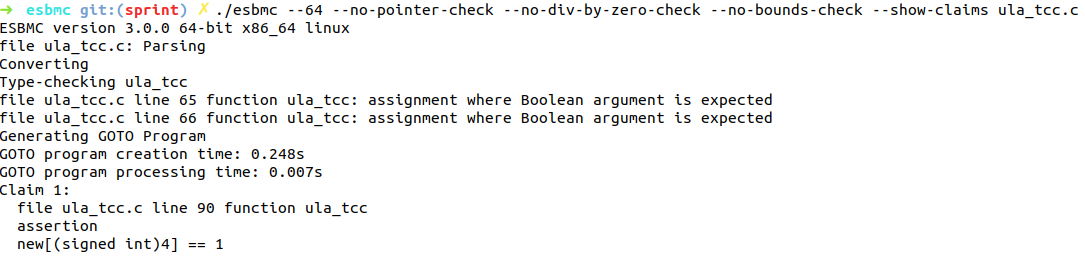
\includegraphics[scale=0.55 ]{Figuras/lista_claim.png}
%	\end{center}
%    \legend{Fonte:Própria}
%\end{figure}

%\par
%Após a listagem das claims com assertivas ser gerada, outra função, indicada na \autoref{fig:analise_claims}, é chamada para verificação de cada claim individualmente. Para cada claim, ocorre a chamada do ESBMC, utilizando as opções \texttt{$--$no-pointer-check}, \texttt{$--$no-div-by-zero-check} e \texttt{$--$no-bounds-check}, juntamente com a opção \texttt{$--$unwind} em que realiza o número de desdobramentos dos laços no código analisado. 

%\par
%Contudo, dependendo da complexidade da assertiva, faz-se necessário aumentar o número de desdobramentos que, por padrão são dez, conforme análise experimentais. A função é chamada na Linha $11$ da \autoref{fig:analise_claims} e após a análise da claim é realizado a busca do resultado e exibição caso seja uma propriedade violada.

%\par
%Desta forma o ESBMC realiza apenas a checagem necessária dentro da assertiva, evitando que outros parâmetros sejam verificados, sem a devida necessidade do mesmo. Ao final de todos os desdobramentos é apresentado o resultado, apresentado na \autoref{fig:resultado}, sendo positiva (sem erros) ou negativa (com violação de propriedades), dependendo da assertiva e do código analisado. Este processo se repete até a lista de assertivas ser finalizada.

%\begin{figure}[H]
%\caption{\label{fig:analise_claims}Pseudocódigo da função de análise das claims.}
%	\begin{center}
%    \begin{minipage}{0.7\textwidth}
%    \begin{lstlisting}       
%VAR
%contador1: inteiro
%contador2: inteiro
%resultado: lista
%
%FUNCAO esbmc_claims: lista, arquivo
%  contador1<-0
%  contador2<-0
%  busca pelo nome da funcao no arquivo
%  ENQUANTO contador < lista FACA
%    saida<-Executa comando de analise da claim numerada na %lista
%    ENQUANTO contador2 < saida
%      Regex busca se a propriedade foi violada
%      SE propriedade foi violada ENTAO
%         Pula para linha da violação
%	       Adiciona o erro ao resultado       
%      FIM-SE  
%    FIM-ENQUANTO
%  FIM-ENQUANTO
%FIM-FUNCAO
%    \end{lstlisting}
%    \end{minipage}
%	\end{center}
%    \legend{Fonte: Própria.}
%\end{figure}

%\begin{figure}[H]
%	\begin{center}
%    \caption{\label{fig:resultado}Imagem de apresentação do resultado da ferramenta.}
%	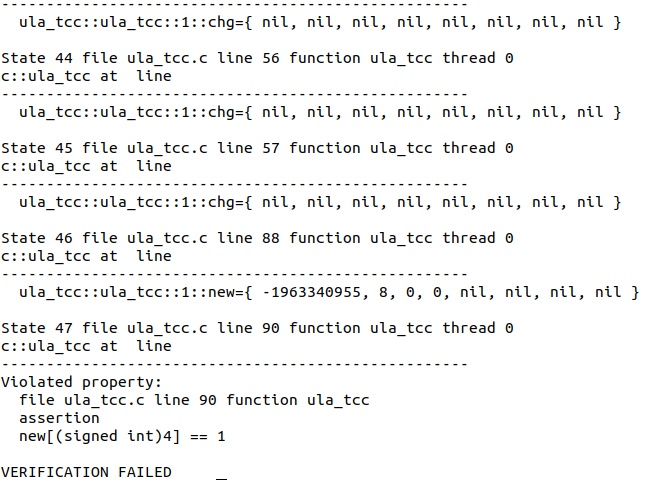
\includegraphics[scale=0.6]{Figuras/erro_assert.png}
%	\end{center}
%    \legend{Fonte:Própria}
%\end{figure}

%++++++++++++++++++++++++++++++++++++++++++++++++++++++++++
%==========================================================
%Método multiplas transformações
%==========================================================
%++++++++++++++++++++++++++++++++++++++++++++++++++++++++++
\subsection{Método multiplas transformações}
%==========================================================
%Visão geral do método multiplas transformações
%==========================================================
%\subsection{Visão geral do método multiplas transformações}
%\par
%O método proposto consiste na tradução de um código em VHDL para linguagem C e posteriormente a análise de deste programa, com base nas assertivas inseridas em um arquivo externo.  Inicialmente o código em VHDL é passado para ferramenta juntamente com outro arquivo contendo as variáveis de entrada, saída, pré-condições e pós-condições. Seguidamente é passado para duas ferramenta de tradução, inicialmente para Verilog que é instrumentado durante a execução e posteriormente traduzido para C. Após as traduções, as pré-condições e pós-condições, conforme o arquivo, são adicionadas ao códigos C e o mesmo é analisado pela ferramenta ESBMC. Caso alguma condição seja violada, o contra exemplo é apresentado ao usuário.

%========================
%Código VHDL e arquivo externo
%========================
\subsubsection{Código VHDL e arquivo externo}
\label{cap:vhdl_assertivas}

A primeira etapa do método consiste inicialmente no código VHDL a ser analisado, juntamente com o arquivo contendo as informações de entradas e saídas do código e também as pré-condições, que são condições que devem ser verdadeira antes da execução de um algum código ou trecho de código, e pós-condições que são condições declaradas e devem ser verdadeiras após a execução de um código ou trecho de código.

\par
O arquivo, \autoref{fig:arquivo_externo}, deve conter todas as variáveis de entrada e saída do código VHDL, apenas o nome da variável em ambos os casos. As variáveis de entrada são declaradas na linha \textbf{INPUT} e as variáveis de saída são declaradas na linha \textbf{OUTPUT}. Nas linhas seguintes são informadas as pré-condições e pós-condições que serão introduzidas ao código em etapas posteriores dos processos.

\begin{figure}[H]
\caption{\label{fig:arquivo_externo} Exemplo de arquivo externo.}
	\begin{center}
    \begin{minipage}{0.8\textwidth}
    \begin{lstlisting}       
INPUT:A==0,B==1,Binvertido==1,Op1==0
OUTPUT:Resultado
PRECONDITION:
POSTCONDITION:Resultado== 0
    \end{lstlisting}
    \end{minipage}
	\end{center}
    \legend{Fonte: Própria.}
\end{figure}

\par
Em comparação ao método anterior, as diferenças consistem principalmente em as assertivas não estarem mais presentes diretamente no código VHDL, desta forma, o mesmo é utilizado apenas nas etapas de tradução. A principal vantagem é a não necessidade de elementos comentados ao código VHDL e com isso o código fica mais legível e também sem a necessidade de modificação ou inserção de trecho para funcionamento da ferramenta em questão.

%===================================
%Tradução de VHDL para C e instrumentações de código
%===================================
\subsubsection{\label{cap:traducao}Tradução de VHDL para C e instrumentações de código}

\par
A primeira etapa é a tradução de código entre VHDL para C, contudo, diferente do demonstrado no primeiro método, onde apenas uma única ferramenta realizava a tradução, nesta nova reformulação do método faz a utilização de duas ferramentas de tradução, inicialmente para Verilog e uma segunda ferramenta faz a tradução para C. Isso possibilita uma um aumento no potencial da tradução, contudo, devido ao uso de duas ferramentas, alguns erros ainda podem ser verificados na tradução.

\par
Devido ao uso das ferramentas, também é necessário mais uma etapa de instrumentação, sendo uma após a tradução para Verilog e outra após a tradução para C. A primeira instrumentação modifica o código para que segunda ferramenta de tradução possa executar a tradução corretamente e a segunda instrumentação adiciona as assertivas, de acordo com o introduzido no arquivo citado na seção anterior. Nas próximas subseções serão explicados com mais detalhes as traduções e as instrumentações.

%================================================
%Tradução para Verilog e instrumentação de código
%================================================
\subsubsubsection{Tradução para Verilog e instrumentação de código}

\par
A primeira ferramenta de tradução utilizada, chamada VHD2Vl\cite{vhd2vl}, realiza a tradução do código VHDL para o código Verilog. O principal motivo de utilizar esta ferramenta deve-se a apresentar melhores resultados na tradução dos códigos, contudo, também apresenta algumas questões a serem observadas nas traduções. 

\par
Entre estas observações esta encontra-se a utilização das estruturas de std\_logic, std\_logic\_vector, integer e boolean. Também permite a utilização clock events das estruturas de controle, como if, elsif, else, case. A ferramenta também permite a instância de módulos no código VHDL, contudo o mesmo é ignorado na tradução o que causa erros de análise. Também é ignorado qualquer assertiva existente no código, tornando assim, mais necessário um arquivo externo com assertivas e condições a serem adicionadas ao texto\cite{vhd2vl}. 


\begin{figure}[H]
\caption{\label{fig:codigo_verilog} Código da \autoref{fig:code_exemplo} traduzido pela ferramenta Vhd2vl.}
	\begin{center}
    \begin{minipage}{0.7\textwidth}
    \begin{lstlisting}
[...]
module Ula_tcc(
input wire A,
input wire B,
input wire Binvertido,
input wire Op1,
output reg Resultado
);
reg and_port;
reg or_port;
reg mux2x1;
  always @(A, B, Binvertido, Op1) begin
    if((Binvertido == 1'b0)) begin
      mux2x1 <= B;
    end
    else begin
      mux2x1 <=  ~B;
    end
    and_port <= A & mux2x1;
    or_port <= A | mux2x1;
    if((Op1 == 1'b0)) begin
      Resultado <= and_port;
    end
    else if((Op1 == 1'b1)) begin
      Resultado <= or_port;
    end
  end
endmodule
    \end{lstlisting}
    \end{minipage}
	\end{center}
    \legend{Fonte: Própria.}
\end{figure}

\par
Contudo, o código conforme apresentado acima, não pode ser traduzido para C, pois está fora do padrão aceito pela ferramenta V2c, que realiza a tradução de verilog para C. Com isso é necessária uma instrumentação de código para que o mesmo possa ser traduzido. Esta instrumentação consiste na alteração dos modo de declaração das variáveis, na alteração de palavras chaves utilizadas no verilog e na busca de elementos que estejam dentro com escopo \textit{always@()}, que contém a arquitetura do código.

\begin{figure}[H]
\caption{\label{fig:codigo_verilog_declaracao} Diferença da declaração das variáveis após a intrumentação.}
	\begin{center}
    \begin{minipage}{0.7\textwidth}
    \begin{lstlisting}
[...]
module Ula_tcc(
input wire A,
input wire B,
input wire Binvertido,
input wire Op1,
output reg Resultado
);
[...]
    \end{lstlisting}
    \end{minipage}
    \legend{(a)}
    \begin{minipage}{0.7\textwidth}
    \begin{lstlisting}
module Ula_tcc(A,B,Binvertido,Op1,Resultado);
input wire A;
input wire B;
input wire Binvertido;
input wire Op1;
output Resultado;
reg Resultado;
[...]
    \end{lstlisting}
    \end{minipage}
    \legend{(b)}
	\end{center}
    \legend{Fonte: Própria.}
\end{figure}

\par
A primeira adaptação a ser feita é na declaração das variáveis. Conforme a \autoref{fig:codigo_verilog_declaracao}(a) apresenta a declaração após a tradução e a \autoref{fig:codigo_verilog_declaracao}(b) apresenta após a instrumentação. As mudanças consistem em o nome das variáveis serem declaradas como uma espécie de parâmetro e logo abaixo seus respectivos tipos, fora do modulo. Outra alteração é com relação ao \textbf{Output reg}, onde primeiro se declara como saída e depois como reg a mesma variável, como apresentado na linha 7 e 8 da \autoref{fig:codigo_verilog_declaracao}(b) em relação a linha 7 da \autoref{fig:codigo_verilog_declaracao}(a). 

\par
Outra alteração necessário é que nenhuma variável seja declarada dentro do modulo Always@(), pois gera a não tradução do código por parte da ferramenta. Com isso toda e qualquer variável que venha a ser utilizado durante a execução do código deve ser declarado antes do modulo always@(), conforme \autoref{fig:codigo_verilog_always}. E outra alteração consiste nas palavras reservadas, visto que verilog utiliza a palavra \textbf{define} para definição de constante. Esta alteração é importante, pois evita que o código seja traduzido de maneira errada. 

\begin{figure}[H]
\caption{\label{fig:codigo_verilog_always} Declaração de variáveis anteriores ao modulo Always@()}
	\begin{center}
    \begin{minipage}{0.7\textwidth}
    \begin{lstlisting}
[...]
reg and_port;
reg or_port;
reg mux2x1;

always @(A, B, Binvertido, Op1) begin
    [...]
endmodule
    \end{lstlisting}
    \end{minipage}
	\end{center}
    \legend{Fonte: Própria.}
\end{figure}

\par

%================================================
%Tradução para Verilog e instrumentação de código
%================================================
\subsubsubsection{Tradução para C e adição das pre-condições e pós-condições.}

\par
A segunda parte da tradução é realizada pela ferramenta V2C \cite{mukherjee2016v2c}. Como citado anteriormente, após a instrumentação no código verilog o mesmo pode ser traduzido para C, conforme apresentado na \autoref{fig:codigo_C}. Após a tradução o código recebe as assertivas e inicializações de variáveis.  

\par
Toda parte de arquitetura do código VHDL após a tradução para C é colocada em uma função de mesmo nome do arquivo. Também é definido uma \textit{struct} que contém as variáveis que foram declaradas como \textit{output} e também variáveis que tenham sido declaradas para serem utilizadas na execução da arquitetura, como os sinais por exemplo. As variáveis de entrada são declaradas na função main() e são repassadas como parâmetros da função. 

\par
A necessidade desta \textit{struct} deve-se ao fato de que estas variáveis podem ter seus valores alterados em tempo de execução. Devido a este fato, variáveis são criadas para armazenar valores antigos e também receber novos valores, como ocorre nas linhas treze, catorze, quinze e dezeseis da \autoref{fig:codigo_C}. Nota-se que estas variáveis possuem o mesmo nome das variáveis da \textit{struct}, com a adição do sufixo \_old. 

\par
Após a etapa de conversão para linguagem C ocorre uma nova etapa de instrumentação de código, onde as assertivas serão introduzidas ao código C. Para isso faz-se necessário a utilização do arquivo de pré-condições e pós-condições passado para ferramenta juntamente com o código VHDL e apresentado na \autoref{fig:arquivo_externo}.  

\begin{figure}[H]
\caption{\label{fig:codigo_C} Código C traduzido após a intrumentação no verilog.}
	\begin{center}
    \begin{minipage}{0.7\textwidth}
    \begin{lstlisting}
#include <stdio.h>
#include <assert.h>
#define TRUE 1
#define FALSE 0
struct state_elements_Ula_tcc{
_Bool Resultado;
_Bool and_port;
_Bool or_port;
_Bool mux2x1;
};
void Ula_tcc(_Bool A, _Bool B, _Bool Binvertido, _Bool Op1, _Bool *Resultado){
  struct state_elements_Ula_tcc  sUla_tcc;
  _Bool Resultado_old;
  _Bool and_port_old;
  _Bool or_port_old;
  _Bool mux2x1_old;
  mux2x1_old = sUla_tcc.mux2x1;
  and_port_old = sUla_tcc.and_port;
  or_port_old = sUla_tcc.or_port;
  Resultado_old = sUla_tcc.Resultado;
  if((unsigned char)Binvertido == 0){
    sUla_tcc.mux2x1 = B;
  }
  else{
    sUla_tcc.mux2x1 = !B;
  }
  sUla_tcc.and_port = A && mux2x1_old;
  sUla_tcc.or_port = A || mux2x1_old;
  if((unsigned char)Op1 == 0){
    sUla_tcc.Resultado = and_port_old;
  }
  else{
    if((unsigned char)Op1 == 1){
      sUla_tcc.Resultado = or_port_old;
    }
  }
}
void main() {
_Bool A;
_Bool B;
_Bool Binvertido;
_Bool Op1;
_Bool Resultado;
Ula_tcc(A, B, Binvertido, Op1, &Resultado);
}
    \end{lstlisting}
    \end{minipage}
	\end{center}
    \legend{Fonte: Própria.}
\end{figure}

\par
Para a instrumentação é necessário a utilização de funções próprias do analisador, neste caso o ESBMC \cite{esbmc} e estas funções são: \textbf{ESBMC\_assume()}, \textbf{\_\_VERIFIER\_nondet\_int()} e \textbf{\_\_VERIFIER\_nondet\_bool()}. A função \textbf{ESBMC\_assume()} permite que uma variável assuma um valor especifico. As funções \textbf{\_\_VERIFIER\_nondet\_int()} e \textbf{\_\_VERIFIER\_nondet\_bool()} modelam valores inteiros e booleanos não deterministicos respectivamente.

\par
A função ESBMC\_assume() é utilizada quando alguma variável foi inicializada no arquivo, desta forma a mesma é inicializada no código. Na linha 1 da \autoref{fig:arquivo_externo} é declarada variável inicializada e das linhas 21 a 24 da \autoref{fig:codigo_C_assert} é utilizado as funções para declaração das variáveis. Desta forma,  estes valores são definidos para aquela variável no tempo de execução da análise. 

\par
A importância das funções \textbf{\_\_VERIFIER\_nondet\_int()} e \textbf{\_\_VERIFIER\_nondet\_bool()} no desenvolvimento do método é evitar que um determinado estado do código não possa ser alcançado, devido a não inicialização de variáveis. Estas funções são utilizadas nas variáveis de entrada não inicializadas e as outras variáveis que não são inputs e nem outputs. Na \autoref{fig:codigo_C_assert}, linhas 48 a 51 apresenta o uso desta função.

\par
Em outras palavras, na instrumentação de código é realizado a adição das assertivas do modelo utilizado no arquivo para o modelo utilizado em linguagem C, além como de outras funções que possam ser utilizados pelo VHDL. Ao final da instrumentação o código C fica disponível para que possa ser dado como entrada para outras ferramentas de verificação de código e não apenas o ESBMC. 

\begin{figure}[H]
\caption{\label{fig:codigo_C_assert} Código C adição das assertivas.}
	\begin{center}
    \begin{minipage}{0.7\textwidth}
    \begin{lstlisting}
#include <stdio.h>
#include <assert.h>
#define TRUE 1
#define FALSE 0
struct state_elements_Ula_tcc{
_Bool Resultado;
_Bool and_port;
_Bool or_port;
_Bool mux2x1;
};
void Ula_tcc(_Bool A, _Bool B, _Bool Binvertido, _Bool Op1, _Bool *Resultado){
  struct state_elements_Ula_tcc  sUla_tcc;
  _Bool Resultado_old;
  _Bool and_port_old;
  _Bool or_port_old;
  _Bool mux2x1_old;
  mux2x1_old = sUla_tcc.mux2x1;
  and_port_old = sUla_tcc.and_port;
  or_port_old = sUla_tcc.or_port;
  Resultado_old = sUla_tcc.Resultado;
  __ESBMC_assume(A==0);
  __ESBMC_assume(B==1);
  __ESBMC_assume(Binvertido==1);
  __ESBMC_assume(Op1==0);
  if((unsigned char)Binvertido == 0){
    sUla_tcc.mux2x1 = B;
  }
  else{
    sUla_tcc.mux2x1 = !B;
  }
  sUla_tcc.and_port = A && mux2x1_old;
  sUla_tcc.or_port = A || mux2x1_old;
  if((unsigned char)Op1 == 0){
    sUla_tcc.Resultado = and_port_old;
  }
  else
    if((unsigned char)Op1 == 1){
      sUla_tcc.Resultado = or_port_old;
    }
    __ESBMC_assert(sUla_tcc.Resultado == 0,"Teste");
}
void main() {
_Bool A;
_Bool B;
_Bool Binvertido;
_Bool Op1;
_Bool Resultado;
A=__VERIFIER_NONDET_BOOL();
B=__VERIFIER_NONDET_BOOL();
Binvertido=__VERIFIER_NONDET_BOOL();
Op1=__VERIFIER_NONDET_BOOL();
Ula_tcc(A, B, Binvertido, Op1, &Resultado);
}
    \end{lstlisting}
    \end{minipage}
	\end{center}
    \legend{Fonte: Própria.}
\end{figure}
%=============================================
%Verificação de assertvas usando model checker
%=============================================
\subsection{\label{sec:verificacao}Verificação de assertivas usando \textit{Model Checker}}

\par
O \textit{model checker} adotado no desenvolvimento de método é o ESBMC~\cite{cordeiro2012smt} na versão $6.0.0$ e conforme explicado na Seção~\ref{cap:bounded}, esta ferramenta recebe como entrada um código C ou C$++$ e também utiliza solucionadores SMT para análise do programa. 

\par
Para verificação pode ser utilizado o métodos de análise, chamado indução-k. A indução-k é o meio principal de verificação, juntamente com o mesmo é adicionado as seguintes opções, estas que o analisador trabalhe diretamente e unicamente com as assertivas, evitando que outros fatores possam ser analisados no código: 
\begin{itemize} 
    \item \textbf{$--$no-pointer-check:} para não realizar a checagem de ponteiros no código; 
    \item \textbf{$--$no-div-by-zero-check:} para não realizar a checagem de divisões por zero no código; e 
    \item \textbf{$--$no-bounds-check:} para não realizar a checagem de array bounds no código. 
\end{itemize} 

\par
\textcolor{red}{Desta forma o ESBMC realiza apenas a checagem necessária dentro da assertiva, evitando que outros parâmetros sejam verificados, sem a devida necessidade do mesmo. O ESBMC utilizando a técnica de indução-k realiza a análise das assertivas em cada código, considerando as pré condições e também os valores determinados para as variáveis dentro o código através do ESBMC\_assume(). Ao final de todos os desdobramentos é apresentado o resultado, sendo positiva (sem erros) ou negativa (com violação de propriedades), dependendo da assertiva e do código analisado.}

\section{Resumo do capitulo}
\textcolor{red}{Neste capitulo foi apresentado os dois métodos de tradução composto pelo método de múltiplas traduções, na qual é utilizado duas ferramentas de tradução, e pelo método de tradução direta que utiliza apenas uma ferramenta e faz a conversão direta de VHDL para linguagem C. Também foi mostrado a ferramenta de análise chamada ESBMC e de que forma ela é utilizada para verificação dos códigos.} 
%------------------------------------------------------------
% Cronograma
%------------------------------------------------------------
%\chapter{CRONOGRAMA}
%\label{chapter:cronograma}
\begin{table}[htbp]
  \centering
  \caption{Cronograma de atividades}
  \label{tab:cronograma}
  \begin{tabularx}{\textwidth}{|X|c|c|c|c|c|}
    \hline
    \textbf{Atividade} & \textbf{Agosto} & \textbf{Setembro} & \textbf{Outubro} & \textbf{Novembro} & \textbf{Dezembro} \\
    \hline
    Revisão da literatura sobre verificação de hardware com assertivas & \(\times\) & \(\times\) & & & \\
    \hline
    Busca e teste de ferramenta para traução de código VHDL para C & \(\times\) & & & & \\
    \hline
    Definição e implementação de assertivas da execução automática da ferramenta & & \(\times\) & \(\times\) & & \\
    \hline
    Adicionar Bounded model checking no método & & \(\times\) & \(\times\) & &  \\
    \hline
    Finalização da implementação das funcionalidades da ferramenta & & & \(\times\) & \(\times\) &  \\
    \hline
    Realização de testes com benchmarks públicos escritos em VHDL & & &  & \(\times\) & \\
    \hline
    Finalização monografia & & & & \(\times\) & \(\times\) \\
    \hline
    Apresentação final & & & &  & \(\times\) \\
    \hline
  \end{tabularx}
\end{table}
% -----------------------------------------------------------
% Resultados -- Pode vir junto com discussão
% -----------------------------------------------------------
\chapter{RESULTADOS EXPERIMENTAIS}
\label{chapter:resultados}
\par
Neste capitulo será apresentado o planejamento, execução e os resultados do método proposto neste trabalho. \textcolor{red}{Serão apresentados dois experimentos neste capitulo, sendo inicialmente um para os métodos de tradução e outro para o método de análise. Desta forma abrangendo todo o método do trabalho. O objetivo destes experimentos é testar as ferramentas utilizadas, assim como descobrir os limites de utilização da mesma.}
%\todo[inline]{Adicionar um breve descrição do planejamento e objetivo do experimento }
%\todo[inline]{Sugiro também uma revisão do português do texto, em relação a acentos.}

\section{Planejamento da avaliação experimental}

\par 
Os testes apresentados neste capitulo tem o objetivo de apresentar o potencial da \textcolor{red}{abordagem do método proposto em relação a tradução de código VHDL para C e análise de código apresentado \autoref{chapter:metodo}. O teste será dividido em duas metade etapas, inicialmente será testado os métodos de tradução, sendo os métodos de transformação direta e de múltiplas sucessões.} Também será analisada o potencial de análise utilizada neste método, demonstrando a performance da mesma com a abordagem que apresentou o melhor resultado de tradução. 

\textcolor{red}{Os teste serão executados em ambiente linux, precisamente o Ubuntu 16.04, utilizando a ferramenta WSL(Windows Subsystem fo Linux). A maquina utilizada para os teste corresponde a um Dell, processador I7 5500U 2,40Ghz, 8GB de memória ram, contendo o sistema operacional Windows 10 64 bit, na versão 1803.}
%\todo[inline]{Está confuso o texto acima, parece que você só vai testar a tradução e não o seu método completo}

%\todo[inline]{Falta descrever o ambiente dos testes, bem como, a versão das ferramentas usadas e onde estão disponíveis. Lembre que os testes devem ser reproduzíveis.}

\par 
Baseado \textcolor{red}{no objetivo de testar o potencial das abordagens de tradução} foram desenvolvidas as seguintes questões de pesquisa para os testes nas abordagens de tradução e nas ferramentas utilizadas: 
\begin{enumerate} 
    \item As ferramentas de tradução de código são capazes de manipular as diferentes estruturas de código VHDL? 
    \item Existem melhorias a serem efetuadas na tradução de código?
%     Caso não traduza, é possível alterar o código de modo que possa ser traduzido? 
    \item Quais são os impactos de uso das ferramentas auxiliares na aplicação do método proposto? 
\end{enumerate} 

\par 
Para o teste a serem realizados na ferramenta de análise ESBMC foram desenvolvidas as seguintes questões de pesquisa: 
%\todo[inline]{Qual o objetivo destes testes?}
\begin{enumerate} 
    \item A ferramenta ESBMC foi capaz de analisar todos os códigos traduzidos de VHDL para C? 
    \item Quais as limitações apresentadas pela ferramenta de análise ESBMC? 
\end{enumerate} 

\par 
Para os testes do método proposto foi utilizado um benchmark composto por 20 códigos escritos em VHDL. Estes códigos são oriundos das seguintes fontes: 

\begin{itemize} 
    \item \textbf{Fonte própria do autor:} $10$ códigos foram desenvolvidos pelo autor para utilização em testes das ferramenta. Estes códigos correspondem a portas lógicas, multiplexadores, entre outros códigos;  
    \item \textbf{ICAS99:} $6$ códigos foram extraídos do benchmark externo ISCAS99. Apresentam um grau de complexidade maior que os códigos do autor, e desta forma buscar os limites das ferramentas. O benchmark está disponível em:
    
    \texttt{http://www.pld.ttu.ee/$\sim$maksim/benchmarks/iscas99/vhdl/}.  
    
    \item \textbf{Benchmark Vhd2vl:} $4$ códigos foram extraídos dos exemplos existente junto com a ferramenta Vhd2vl. Estes códigos apresentam diversos graus de complexidade, buscando analisar não somente as limitações desta ferramenta, mas se é possível que estes códigos sejam analisados ao final. 
\end{itemize} 

\todo[inline]{Descrever para o ICAS99 e Vhd2vl, sobre o que são os códigos.}

\par
\textcolor{red}{Conforme citado anteriormente, os teste serão divididos em duas etapas, inicialmente o teste será realizado apenas com os métodos de tradução. Será passado para os métodos o benchmark de 20 códigos citados acima e é observado qual das abordagens demonstrou o melhor desempenho, ou seja, qual método foi capaz de traduzir mais códigos de VHDL para C. Cada método de tradução será executado conforme apresentado no \autoref{chapter:metodo}.}

\par
\textcolor{red}{Para as traduções serão testadas 3 ferramentas, sendo duas ferramentas para o método de múltiplas transformações, sendo elas a ferramenta Vhd2vl, na versão X disponível no site, que realiza a tradução de VHDL para Verilog. E a ferramenta V2c, na versão e disponível no site, que realiza a tradução de Verilog para C. No método de tradução direta apenas a ferramenta V2c que realiza a tradução de VHDL para C. É importante ressaltar que apesar do mesmo nome, V2c, os métodos apresentam ferramentas diferentes, com usos diferentes.}

\par
\textcolor{red}{A segunda etapa de testes será o teste da ferramenta de análise ESBMC. Os testes serão realizados em conjunto com o método de tradução que obteve o melhor resultado, ou seja, o método que apresentou o maior conjunto de códigos traduzidos será utilizado em conjunto com a ferramenta ESBMC para o teste da ferramenta. A ferramenta ESBMC está disponível no site \textit{www.esbmc.com} e será utilizado esta na versão 6.0.0 desta ferramenta.}

\par
\textcolor{red}{O motivo desta abordagem de teste ter sido utilizada deve-se ao fato de uma quantidade maior de códigos ser utilizada para os testes, além de que os melhores resultados, tecnicamente deve apresentar os melhores códigos. Para os testes os códigos traduzidos para linguagem C terão assertivas inseridas aos códigos e a ferramenta deve ser capaz de encontrar estas assertivas, mas também verificar se alguma propriedade destas assertivas foi violada ou não.}
\par 
%Para os testes da ferramenta ESBMC foram utilizados os códigos traduzido pelas abordagens, contudo apenas os códigos da abordagem que teve o melhor desempenho durante o teste, pelo fato que se esperasse que a melhor abordagem tenha uma quantidade maior de códigos traduzidos\todo{Este texto está muito confuso, não entendi :(}. 

\par 
%O motivo da utilização de outras fontes de benchmark é testar o real desempenho do método proposto, testando não apenas com códigos simples, como porta lógicas ou multiplexadores, mas também códigos que apresentem outras estruturas do VHDL, além das utilizadas no benchmark do autor, em outras palavras, em códigos mais complexo, as chance são maiores da ferramenta não conseguir realizar a tradução do código\todo{Está meio retudante, sugiro melhorar}. 

\par 
%Os testes foram realizados da seguinte maneira, era passado para ambas as abordagens os mesmos códigos, de acordo com o modo funcionamento de cada operação de tradução, também foi verificado se o código traduzido era reconhecido pela ferramenta ESBMC. Logo,  verificado se todas as etapas foram concluídas, caso contrário é analisado em qual etapa o erro foi gerado e a possível causa do erro. Nesta etapa não foi introduzida assertiva, visando apenas testar a capacidade de tradução ser realizada pelas ferramentas.  

\par 
%Visando analisar a capacidade da verificação do código traduzido, somente a melhor abordagem foi selecionada e a ela inserida as assertivas aos códigos que foram traduzidos a linguagem C por esta abordagem. Também foi apresentada um cálculo de tempo tanto para tradução quanto para o tempo que foi necessário para análise de código. 

%\todo[inline]{Melhorar texto acima.}

%======================================
%Apresentação dos resultados dos testes
%======================================
\section{Execução e análise dos resultados}

\textcolor{red}{Nesta sessão será apresentado os resultados proveniente dos testes explanados na sessão anterior. Primeiramente será apresentado os resultados dos métodos de tradução e posteriormente será apresentado os resultados relacionados a ferramenta de análise ESBMC.}
%\todo[inline]{Adicionar um texto de introdução a seção}

\subsection{Testes realizados nas abordagens de tradução}

Após a execução dos benchmarks, no teste dos métodos de tradução, os
%\todo{quais de tradução ou verificação?} 
resultado da obtidos são apresentados na \autoref{tab:tabela_resultado}, formada pelas colunas: \textbf{Id} que é uma identificação para cada código; \textbf{Nome do código}; \textbf{Abordagem 01} que representa a abordagem de multiplas traduções; \textbf{vhd2vl} que apresenta o status para tradução da ferramenta vhd2vl; \textbf{v2c} para o status da ferramenta de tradução; \textbf{Abordagem 02} que representa a abordagem de transformação direta; \textbf{v2c} que representa o status de tradução da ferramenta v2c.

\par
A ferramenta ESBMC também foi adicionada como forma de parâmetro para testar as traduções realizadas, de modo a saber se algum estrutura em C gerada pelas traduções não seria reconhecida, visto que o ESBMC será utilizado no método proposto como o verificador de pós-condições. Vale lembrar que a ferramenta V2C utilizada na \textbf{Abordagem 01} é diferente da ferramenta utilizada na \textbf{Abordagem 02}. A primeira realiza traduções de Verilog para C
%\todo{Como ocorre a tradução de VHDL para Verilog}
, enquanto a segunda realiza de VHDL para C. 

\begin{table}[H]
\centering
\caption{Resultados das abordagens de tradução}
\label{tab:tabela_resultado}
\begin{tabular}{|c|c|c|c|c|c|c|}
\hline
\multicolumn{7}{|c|}{\textbf{Benchmark Oficial}} \\ \hline
\multirow{2}{*}{\textbf{ID}} & \multirow{2}{*}{\textbf{Nome arquivo}} & \multicolumn{3}{c|}{\textbf{Abordagem 01}} & \multicolumn{2}{c|}{\textbf{Abordagem 02}} \\ \cline{3-7} 
 &  & \textbf{VHD2VL} & \textbf{V2C} & \multicolumn{1}{l|}{\textbf{ESBMC}} & \textbf{V2C} & \multicolumn{1}{l|}{\textbf{ESBMC}} \\ \hline
1 & AND\_ent.vhd & SIM & SIM & SIM & SIM & SIM \\ \hline
2 & XOR\_ent.vhd & SIM & SIM & SIM & SIM & SIM \\ \hline
3 & ifchain.vhd & SIM & SIM & SIM & NÃO & - \\ \hline
4 & B01.vhd & SIM & SIM & SIM & SIM & NÃO \\ \hline
5 & B06.vhd & SIM & SIM & SIM & SIM & NÃO \\ \hline
6 & B10.vhd & SIM & SIM & SIM & SIM & NÃO \\ \hline
7 & Comb1.vhd & SIM & SIM & SIM & SIM & SIM \\ \hline
8 & FlipFlop\_D.vhd & SIM & SIM & SIM & SIM & SIM \\ \hline
9 & seq1.vhd & SIM & SIM & SIM & SIM & SIM \\ \hline
10 & Ula\_tcc.vhd & SIM & SIM & SIM & SIM & SIM \\ \hline
11 & dff.vhd & SIM & SIM & SIM & SIM & SIM \\ \hline
12 & mux\_2to1\_top.vhd & SIM & SIM & SIM & SIM & SIM \\ \hline
13 & b02.vhd & SIM & SIM & SIM & SIM & NÃO \\ \hline
14 & b03.vhd & SIM & SIM & SIM & SIM & NÃO \\ \hline
15 & b09.vhd & SIM & SIM & SIM & SIM & NÃO \\ \hline
16 & counters.vhd & SIM & NÃO & - & NÃO & - \\ \hline
17 & ifchain2.vhd & SIM & SIM & NÃO & NÃO & - \\ \hline
18 & mem.vhd & SIM & NÃO & - & NÃO & - \\ \hline
19 & Nand\_ent.vhd & SIM & SIM & SIM & SIM & SIM \\ \hline
20 & Nor\_ent.vhd & SIM & SIM & SIM & SIM & SIM \\ \hline
\end{tabular}
\end{table}

\par
Entre os códigos utilizado no benchmark, os seguintes resultados da \textbf{Abordagem 01} foram obtidos:
\begin{itemize}
    \item $20$ códigos passaram pela ferramenta Vhd2vl. Contudo, os códigos com ID $16$ e $18$ não foram inteiramente traduzidos devido a ferramenta não ser capaz de fazer a link entre as variáveis declaradas; 
    \item Dos $20$ códigos foram traduzidos para Verilog e instrumentados $18$ que foram traduzidos para linguagem C. Os códigos não, citado anteriormente, temos que o código com ID $17$ apresentou uma especie de "lixo", como se o tradutor não reconhecesse a estrutura no verilog durante a tradução para C.
    \item Dos $18$ códigos, $17$ códigos foram reconhecidos pelo ESBMC. O código com ID $17$ apresentou erros, como citado acima o que ocasionou operação abortada pelo analisador ESBMC.
\end{itemize}

%====================================================
\par
Entre os códigos utilizado no benchmark, os seguintes resultados da \textbf{Abordagem 02} foram obtidos:
\begin{itemize}
    \item Dos $20$ códigos, apenas $16$ foram traduzidos pela ferramenta v2c
    %\todo{O que significa?} 
    pela ferramenta. Isso deve-se a alguma declaração de variável inteira nos códigos e/ou devido a estrutura \texttt{downto} no VHDL apresentar erro na tradução; e
    \item Dos $16$ códigos traduzidos e instrumentados, apenas $10$ foram aceitos pela ferramenta de analise do ESBMC.
\end{itemize}

Com base nestes resultados apresentados é possível destacar que o método de múltiplas traduções (Abordagem 01) apresentou um desempenho melhor na tradução dos códigos. Vale ressaltar que é uma melhoria na tradução, visto que o método de tradução simples foi utilizado no desenvolvimento do TCC 1. Contudo, uma maior quantidade de ferramentas pode aumentar a complexidade da tradução e gerar mais erros de sintaxe.

\subsection{Análise da verificação de código}
Como citado no inicio do capítulo, a apresentação dos resultados da ferramenta ESBMC seria realizado com a abordagem que tivesse a melhor desempenho no teste de tradução, sendo o caso, o método de múltiplas transformações. Foram utilizados $17$ códigos para o teste da ferramenta de verificação ESBMC, todos os códigos apresentam as pré (usando a função \texttt{\_\_VERIFIER\_assume} do ESBMC) e pós condições  em \texttt{asserts}. 
% adicionadas e o resultado a ser alcançado, 
Os resultados esperados na verificação com o ESBMC são \texttt{TRUE}, a assertiva não foi violada, ou \textit{FALSE} caso contrário. \textcolor{red}{Nas tabelas \autoref{tab:tabela_verificacao_1} e \autoref{tab:tabela_verificacao_2} apresentam os resultados dos teste e também o tempo de cada operação.}

\par
\textcolor{red}{A \autoref{tab:tabela_verificacao_1} apresenta \textbf{ID}, \textbf{Nome do código}, \textbf{Tradução verilog}, se o código foi capaz de ser traduzido, \textbf{Tempo de tradução} desde o VHDL até a linguagem C, \textbf{Pre-condição} e \textbf{Assume}. A tabela ainda apresenta dois termos, sendo VNB e EAE. O primeiro é a sigla para \_\_VERIFIER\_NONDET\_BOOL() que gerar valores não deterministicos para ser utilizado durante o experimento. O segundo é a sigla para \_\_ESBMC\_assume() que é uma função da ferramenta de análise utilizada para aplicar valores a determinadas variáveis.} 

\par
\textcolor{red}{A \autoref{tab:tabela_verificacao_2} apresenta \textbf{ID}, \textbf{Pós-condição}, \textbf{Resultado esperado} que é o resultado a ser esperado pela ferramenta de análise, de acordo com as pre e pós condições, e \textbf{Tempo de execução}. Assim como a tabela anterior, aqui é apresentado a sigla EAT para \_\_ESBMC\_assert(), a qual é utilizada para adicionar as assertivas ao código VHDL.}

\begin{table}[H]
\centering
\caption{Resultado da ferramenta de análise}
\label{tab:tabela_verificacao_1}
\begin{tabular}{|l|l|l|l|l|l|}
\hline
\multicolumn{6}{|c|}{BENCHMARK OFICIAL} \\ \hline
ID & \multicolumn{1}{c|}{Nome do Código} & \multicolumn{1}{c|}{\begin{tabular}[c]{@{}c@{}}Tradução \\ verilog\end{tabular}} & \multicolumn{1}{c|}{\begin{tabular}[c]{@{}c@{}}Tempo \\ de \\ tradução\end{tabular}} & \multicolumn{1}{c|}{Pre-condição} & \multicolumn{1}{c|}{Assume} \\ \hline
1 & AND\_ent.vhd & SIM & 0m0.231s & \begin{tabular}[c]{@{}l@{}}X=VNB; \\ Y=VNB\end{tabular} & \begin{tabular}[c]{@{}l@{}}EAE(x==TRUE);\\ EAE(y==TRUE);\end{tabular} \\ \hline
2 & XOR\_ent.vhd & SIM & 0m0.161s & \begin{tabular}[c]{@{}l@{}}X=VNB; \\ Y=VNB\end{tabular} & \begin{tabular}[c]{@{}l@{}}EAE(x==FALSE); \\ EAE(y==TRUE);\end{tabular} \\ \hline
3 & B01.vhd & SIM & 0m7.008s & \begin{tabular}[c]{@{}l@{}}line1=VNB; \\ line2=VNB; \\ reset=VNB; \\ clock=VNB;\end{tabular} & \begin{tabular}[c]{@{}l@{}}EAE(reset == 0); \\ EAE(line1 == 0); \\ EAE(line2 == 0); \\ EAE(stato\_old == 1);\end{tabular} \\ \hline
4 & B06.vhd & SIM & 0m3.431s & \begin{tabular}[c]{@{}l@{}}eql=VNB;\\ clock=VNB; \\ reset=VNB; \\ cont\_eql=VNB;\end{tabular} & \begin{tabular}[c]{@{}l@{}}EAE(reset == 0); \\ EAE(cont\_eql == 1); \\ EAE(eql == 1);  \\ EAE(state\_old == 0);\end{tabular} \\ \hline
5 & Comb1.vhd & SIM & 0m1.292s & \begin{tabular}[c]{@{}l@{}}a=VNB; \\ b=VNB; \\ c=VNB; \\ d=VNB; \\ e=VNB;\end{tabular} & - \\ \hline
6 & FlipFlop\_D.vhd & SIM & 0m0.677s & \begin{tabular}[c]{@{}l@{}}D=VNB; \\ CLK=VNB; \\ RST=VNB;\end{tabular} & EAE(RST==1); \\ \hline
7 & seq1.vhd & SIM & 0m0.958s & \begin{tabular}[c]{@{}l@{}}in1=VNB; \\ in2=VNB; \\ reset=VNB;\end{tabular} & \begin{tabular}[c]{@{}l@{}}EAE(reset == 1); \\ EAE(in1 == 0); \\ EAE(in2 == 0);\end{tabular} \\ \hline
8 & Ula\_tcc.vhd & SIM & 0m0.905s & \begin{tabular}[c]{@{}l@{}}A=VNB; \\ B=VNB; \\ Binvertido=VNB; \\ Op1=VNB;\end{tabular} & \begin{tabular}[c]{@{}l@{}}EAE(A==0); \\ EAE(B==1); \\ EAE(Binvertido==0); \\ EAE(Op1==0);\end{tabular} \\ \hline
9 & dff.vhd & SIM & 0m0.479s & data\_in=VNB; & EAE(data\_in==FALSE); \\ \hline
10 & mux\_2to1\_top.vhd & SIM & 0m0.585s & \begin{tabular}[c]{@{}l@{}}w0=VNB; \\ w1=VNB; \\ s=VNB;\end{tabular} & \begin{tabular}[c]{@{}l@{}}EAE(w0 == TRUE); \\ EAE(w1 == FALSE); \\ EAE(s == FALSE);\end{tabular} \\ \hline
11 & b02.vhd & SIM & 0m3.007s & \begin{tabular}[c]{@{}l@{}}reset=VNB \\ clock=VNB \\ linea=VNB;\end{tabular} & \begin{tabular}[c]{@{}l@{}}EAE(reset == 0); \\ EAE(linea == 0); \\ EAE(stato\_old == 1);\end{tabular} \\ \hline
12 & Nand\_ent.vhd & SIM & 0m0.365s & \begin{tabular}[c]{@{}l@{}}X=VNB; \\ Y=VNB;\end{tabular} & \begin{tabular}[c]{@{}l@{}}EAE(x==TRUE); \\ EAE(y==TRUE);\end{tabular} \\ \hline
13 & Nor\_ent.vhd & SIM & 0m0.386s & \begin{tabular}[c]{@{}l@{}}X=VNB; \\ Y=VNB;\end{tabular} & \begin{tabular}[c]{@{}l@{}}EAE(x==TRUE); \\ EAE(y==TRUE);\end{tabular} \\ \hline
\end{tabular}
\end{table}

\begin{table}[H]
\centering
\caption{Resultado da ferramenta de análise}
\label{tab:tabela_verificacao_2}
\begin{tabular}{|l|l|l|l|}
\hline
\multicolumn{4}{|c|}{BENCHMARK OFICIAL} \\ \hline
ID & \multicolumn{1}{c|}{Pós-condição} & \multicolumn{1}{c|}{\begin{tabular}[c]{@{}c@{}}Resultado \\ esperado\end{tabular}} & \multicolumn{1}{c|}{\begin{tabular}[c]{@{}c@{}}Tempo \\ de \\ execução\end{tabular}} \\ \hline
1 & EAT(sAND\_ent.f==TRUE); & TRUE & 0m1.571s \\ \hline
2 & EAT(sAND\_ent.f==TRUE); & TRUE & 0m0.996s \\ \hline
3 & EAT(sb01.outp==0\&\&sb01.overflw==FALSE); & TRUE & 0m2.127s \\ \hline
4 & EAT(sb06.ackout==FALSE\&\&sb06.enable\_count==FALSE); & TRUE & 0m2.017s \\ \hline
5 & EAT(h==a\textasciicircum{}!(b \&\& c)); & FALSE & 0m1.367s \\ \hline
6 & EAT(sFlipFlop\_D.Q==D); & FALSE & 0m1.050s \\ \hline
7 & EAT(sseq1.out==TRUE); & FALSE &  \\ \hline
8 & EAT(sUla\_tcc.Resultado==0); & TRUE & 0m3.284s \\ \hline
9 & EAT(sdff.data\_out==FALSE); & TRUE & 0m2.417s \\ \hline
10 & EAT(smux\_2to1\_top.f==TRUE); & TRUE & 0m2.334s \\ \hline
11 & EAT(sb02.u==TRUE); & FALSE & 0m2.086s \\ \hline
12 & EAT(sNAND\_ent.f==TRUE); & FALSE & 0m1.106s \\ \hline
13 & EAT(sAND\_ent.f==TRUE); & FALSE & 0m0.774s \\ \hline
\end{tabular}
\end{table}

\par
Conforme apresentados a ferramenta ESBMC foi capaz de localizar as assertivas e encontrar o resultado conforme o esperado. A mesma também apresentou tempos baixos tanto de tradução quanto na análise, mesmo nos códigos mais simples. O que configura uma boa atuação da ferramenta no contexto ao qual a mesma foi aplicada.

%\todo[inline]{Descrever as opção usada no ESBMC, bem como a qual técnica de verificação foi adotada}
\textcolor{red}{Foi utilizado no teste as seguintes a técnica de indução-k e as opções --no-pointer-check na qual não realiza a checagem de ponteiros, --no-div-by-zero-check na qual não realiza a checagem de divisão por zero e no-bounds-check na qual não realiza a checagem de array bounds, conforme apresentado na \autoref{sec:verificacao}.} 

%\todo[inline]{Descrever o que pode ser feito para melhorar a verificação.}
\par
\textcolor{red}{Quanto melhor a tradução realizada, melhor será a verificação do código. Novas técnicas podem ser implementadas ao métodos visando a melhorias da verificação, por exemplo, inicialmente foi utilizado a técnica de \textit{Bounded Model Checking} no método, contudo a utilização da indução-k, que apresenta a técnica de BMC juntamente com técnica de desdobramento de loop\cite{gadelhaesbmc}, aumentou a qualidade na verificação dos códigos.}

\section{Resumo do capitulo}
\par
\textcolor{red}{Neste capitulo foi apresentado os resultados das duas abordagens de tradução mostrando que o método de múltiplas traduções teve um desempenho melhor que o método de tradução direta, apresentando uma quantidade maior de códigos traduzidos e reconhecidos pela ferramenta de análise. Também foi mostrado o resultado da ferramenta de análise com alguns códigos resultando da transformação de múltiplas transformações para demonstrar o desempenho da ferramenta.}
%\chapter{DISCUSSÃO}

% -----------------------------------------------------------
% Conclusão
% -----------------------------------------------------------
\chapter{CONSIDERAÇÕES FINAIS E TRABALHOS FUTUROS}
\label{chapter:consideracoes}
O trabalho aborda o desenvolvimento de um método para análise de circuitos lógicos descrito em VHDL através da aplicação de técnica de transformação de código e a técnica \textit{Bounded Model Cheking}. Este método tem como objetivo de explorar os estados alcançáveis no circuito, e dessa forma identificar erros que possam resultar em mal funcionamento do sistema.

\par
Entre as dificuldade encontradas, a principal está ligada a etapa de tradução de código. Devido a ferramenta utilizada inicialmente conter diversas limitações e  a mesma diminui a eficácia da ferramenta, pois a quantidade de estruturas que podem ser utilizadas é limitada e com isso limitando também o processo de criação de circuitos lógicos.

\par
Para trabalhos futuros é necessário buscar uma nova ferramenta ou método de tradução que tenha uma gama maior de tradução, seja em estruturas ou palavras reservadas, deste forma o método desenvolvido torna-se mais eficiente e gerando uma menor intervenção do usuário no código VHDL. A melhoria na tradução de código também beneficia a geração das assertivas automaticamente, pois com uma gama maior de estruturas suportadas, mais assertivas podem ser geradas.

\par
Além disso a geração automática das assertivas é outro ponto abordado, visto que na etapa atual ainda não foi implementado. Este recurso visa da liberdade ao desenvolvedor promovendo de maneira automática os teste sobre o código, não necessitando que uma intervenção, tornando a inserção manual apenas em casos específicos de testes.

 
%------------------------------------------------------------
%Apendice A
%------------------------------------------------------------
\chapter{Apêndice A}
\section{\label{sec:ApendiceA}Revisão sistemática}
\par
A revisão sistemática consiste é um método de identificação, análise e interpretação de pesquisas relevantes em determinada área ou questão de pesquisa. Para execução da revisão sistemática se requer um esforço maior, em comparação às pesquisas tradicionais, sendo necessário seguir uma sequência de passos metodológicos sobre a área ou questão de pesquisa ao qual deseja ser feita a pesquisa~\cite{kitchenham2004procedures}.

\par
Para a execução da revisão sistemática, é necessário um esforço considerável, se comparado a uma revisão informal a literatura. Enquanto que a revisão de literatura informal é conduzida de forma \textit{ad-hoc}, sem planejamento e critérios de seleção estabelecidos a priori, a revisão sistemática requer um protocolo formal bem definido, com uma sequência de passos metodológicos, para conduzir uma pesquisa sobre o tema ao qual deseja-se realizar a pesquisa~\cite{MafraTravassos}.

\par
A aplicação da revisão sistemática requer que seja seguido um conjunto bem definido e sequencial de passos, seguindo um protocolo de pesquisa desenvolvido previamente. Através deste método é possível realizar uma extensa pesquisa, contemplando uma grande quantidade de informações sobre o assunto pesquisado~\cite{MafraTravassos}. Este protocolo é construído considerando um tema específico que representa o elemento central da investigação, onde os passos da pesquisa, as estratégias definidas para coletar as evidências e o foco das questões de pesquisa são definidas explicitamente, de tal forma que outros pesquisadores sejam capazes de reproduzir o mesmo protocolo de pesquisa~\cite{biolchini2005systematic}.

\par
Segundo \citeonline{MafraTravassos}, o processo para a condução de revisões sistemáticas envolve três etapas:
\begin{enumerate}
  \item \textbf{Planejamento da Revisão:} os objetivos da pesquisa são listados e o protocolo da revisão é definido.
  \item \textbf{Condução da Revisão:}nesta atividade, as fontes para a revisão sistemática são selecionadas, os estudos primários são identificados, selecionados e avaliados de acordo com os critérios de inclusão, exclusão, e de qualidade estabelecidos durante o protocolo da revisão.
  \item \textbf{Análise dos Resultados:} os dados dos estudos são extraídos e sintetizados para análise e apresentação dos resultados.
\end{enumerate}

\par
Vale ressaltar que como o objetivo deste trabalho é realizar um estudo exploratório de caracterização de área podemos dizer que esta revisão sistemática se caracteriza como uma quasi-sistemática~\cite{travassos2008environment}, pois segue o mesmo processo da revisão sistemática e preserva o rigor e mesmo formalismo para as fases metodológicas de elaboração de protocolo e execução da revisão, mas sem a aplicação de uma meta-análise a princípio, que pode ser aplicada posteriormente.

%==========================================================
%PLANEJAMENTO DA REVISÃO SISTEMÁTICA
%==========================================================
\subsection{Planejamento da Revisão Sistemática}

\par
\textbf{Objetivo:} Este estudo tem o objetivo esquematizado a partir da estrutura do paradigma GQM (do ingles \textit{Goal,Question and Metric})\cite{basili1994experience}.

\begin{table}[h!]
\centering
\label{}
\begin{tabularx}{\textwidth}{|l|X|}
\hline
Analisar & Publicações científicas através de um estudo baseado em revisão sistemática \\ \hline
Com propósito de & Identifica-las \\ \hline
Com relação as & Vantagens e desvantagens da utilização de assertiva e transformações de código na verificação do código na linguagem de descrição VHDL \\ \hline
Do ponto de vista do & Pesquisador \\ \hline
No contexto & Acadêmico ou industrial para verificação de assertivas na linguagem de descrição VHDL \\ \hline
\end{tabularx}
\caption{Objetivo do estudo utilizando o paradigma GQM}
\end{table}

\par
\textbf{Formulação da Pergunta:} Buscamos respostas para as seguintes perguntas:
\begin{itemize}
\item \textbf{Q1:} Quais são os métodos para verificação de circuitos lógicos descritos na linguagem de programação VHDL?
	\begin{itemize}
	\item \textbf{Q1.1:} Foi desenvolvido e está disponível alguma ferramenta para aplicação do método?
	\item \textbf{Q1.2:} Qual a técnica de exploração de estados para circuitos lógicos?
	\item \textbf{Q1.3:} O método proposto é baseado em técnicas de verificação de software?
	\item \textbf{Q1.4:} Como o método proposto valida pré e pós condições no programa?
	\item \textbf{Q1.3:} Foi utilizado algum \textit{benchmark} de programas em VHDL para experimentação e o mesmo encontra-se disponível?
	\item \textbf{Q1.4:} Quais as perspectivas futuras para melhorar da aplicação do método proposto?
	\end{itemize}
\end{itemize}

\par
\textbf{Escopo da pesquisa:}Na delimitação do escopo da pesquisa foram estabelecidos critérios, buscando garantir a viabilidade da execução, acessibilidade dos dados e abrangência do estudo realizado. A pesquisa dar-se-á a partir de bibliotecas digitais através das suas respectivas máquinas de busca e, quando os dados não estiverem disponíveis eletronicamente, através de consultas manuais.

\par
\textbf{Critérios de Seleção de Fontes.} Para as bibliotecas digitais é desejado:
\begin{itemize}
  \item Possuir uma máquina de busca que permita o uso de expressões lógicas ou mecanismo equivalente.
  \item Incluir em sua base, publicações de exatas ou correlatas que possuam relação direta com o tema a ser pesquisado
  \item As máquinas de busca deverão permitir a busca no texto completo das publicações.
\end{itemize}

Segundo \citeonline{rocha2015verificaccao}, os mecanismos de busca utilizados devem garantir resultados únicos através da busca de um mesmo conjunto de palavras-chaves (\textit{string} de busca). Quando isto não for possível, deve-se estudar e documentar uma forma de minimizar os potenciais efeitos colaterais desta limitação.

\textbf{Métodos de Busca das Publicações.} As fontes digitais foram acessadas via Web, através de expressões de busca pré-estabelecidas. A biblioteca digital consultada foi a Scopus, acessível em http://www.scopus.com. Segundo \citeonline{Elsevier}, a Scopus é uma das maiores bases de dados de resumos e citações da literatura de pesquisa \textit{peer-reviewed} com mais de $22,800$ títulos de mais de $5,000$ editoras internacionais abrangendo as áreas de tecnologia, medicina, artes, ciências sociais e com atualizações diárias. Entre as editoras podemos citar: Springer \cite{Springer}; IEEE Xplore Digital Library \cite{IEEE};ACM Digital Library \cite{ACM} ; ScienceDirect/Elsevier \cite{B.V}; Wiley Online Library \cite{Sons}; dentre outras.

\textbf{\textit{String} de Busca.} A \textit{string} de busca foi definida segundo o padrão PICO (do inglês \textit{Population, Intervention, Comparison, Outcomes}) \cite{kitchenham2009systematic}, conforme a estrutura abaixo:
\begin{itemize}
	\item População: Trabalhos publicados em conferências e periódicos que relacionam verificação de propriedades de circuitos lógicos em códigos para a descrição de hardware.

	\item Intervenção: Verificação de propriedades relacionadas a verificação de circuitos para as diferentes estruturas das linguagens de descrição de hardware;

	\item Comparação: análise de cobertura e suporte das abordagens identificadas para a verificação de propriedades das linguagens de descrição de hardware;

	\item Resultados: a partir da descrição das abordagens pretende-se verificar a cobertura que cada abordagem apresenta na manipulação das diferentes estruturas da linguagem de descrição de hardware para a verificação de propriedades baseada em assertivas.
\end{itemize}

Segundo \citeonline{rocha2015verificaccao}, como este estudo representa um estudo de mapeamento/caracterização, a string de busca foi definida de acordo com dois aspectos: População e Intervenção, como é apresentado na estrutura abaixo. Posteriormente esta mesma \textit{string} de busca será executada na biblioteca Scopus para busca de artigos e publicações de modo a gerar uma interseção entre população e intervenção.
\begin{itemize}
\item População: publicações que fazem referência a verificação de propriedades de circuitos lógicos e sinônimos:
	\begin{itemize}
	\item \textbf{Palavras-chaves:} "circuit checker" OR "circuit verification" OR "contract based verification" OR "code analysis" OR "static analysis" OR "dynamic analysis" OR "safety verification" OR "RTL analysis" OR "program analysis" OR "property verification" OR "formal verification" OR "model checking" OR "model checker" OR "hardware checker" OR "hardware verification" OR "validity checker" OR "hardware assertion" OR "assertion checker" OR "assert verification" OR "assertion-based verification" OR "assertion based verification" OR "assertion-based design" OR "bit level verification"
	\end{itemize}
\item Intervenção: Verificação de circuitos e sinônimos:
	\begin{itemize}
	\item \textbf{Palavras-chaves:}"hardware statement" OR "hardware code" OR "hardware source code" OR "hardware semantics" OR "hardware property" OR "logical gates" OR "sequential circuit" OR "parallel circuit" OR "real circuits" OR "complex circuits" OR "control circuitry" OR ”software netlist” OR “hardware emulation” OR “silicon debug”
	\end{itemize}
\end{itemize}

%==========================================================
%PROCEDIMENTOS DE SELEÇÃO E CRITERIOS
%==========================================================
\subsubsection{Procedimentos de Seleção e Critérios}

\par
A estratégia de busca será aplicada por um pesquisador para identificar as publicações em potencial. A seleção das publicações dar-se-á em 2 etapas, conforme apresentado a seguir.

\begin{enumerate}
\item \textbf{Seleção e catalogação preliminar dos dados coletados:} A seleção preliminar das publicações será feita a partir da aplicação da string de busca na biblioteca Scopus, o resultado desta busca corresponde a seleção preliminar. Todas as publicações serão armazenadas para análise posterior;

\item \textbf{Seleção dos dados relevantes - [1 filtro]:} A seleção preliminar com o uso da expressão de busca não garante que todo o material coletado seja útil no contexto da pesquisa, pois a aplicação das expressões de busca é restrita ao aspecto sintático. Por isso, é necessário a criação de filtros de exclusão e inclusão, de modo a classificar os artigos e publicações que se enquadram no contexto da pesquisa realizada. Nesta etapa apenas serão lidos o título, abstracts, e palavras-chaves e classificar de acordo com os filtros, ou seja, se será aceito ou excluído. Devem ser excluídas as publicações contidas no conjunto preliminar que:
	\begin{itemize}
	\item \textbf{CE1-01:} Não serão selecionadas publicações em que as palavras-chave da busca não apareçam no título, resumo e/ou texto da publicação (excluem-se os seguintes campos: as seções de agradecimentos, biografia dos autores, referências bibliográficas e anexas).
	\item \textbf{CE1-02:} Não serão selecionadas publicações em que descrevam e/ou apresentam ‘keynote speeches’, tutoriais, cursos e similares.
	\item \textbf{CE1-03:} Não serão selecionadas publicações em que o contexto das palavras-chave utilizadas no artigo leve a crer que a publicação não cita uma abordagem para verificação/validação de códigos para descrição de hardware.   
	\item \textbf{CE1-04:} Não serão selecionadas publicações em que o contexto das palavras-chave utilizadas no artigo leve a crer que a publicação não cita uma abordagem para verificação de código de descrição de hardware baseado em assertivas ou propriedades de verificação de hardware.
\end{itemize}

Podem ser incluídas apenas as publicações contidas no conjunto preliminar que:

	\begin{itemize}
	\item \textbf{CI1-01:}Podem ser selecionadas publicações em que o contexto das palavras-chave utilizadas no artigo leve a crer que a publicação cita uma abordagem para verificação de código de descrição de hardware baseado em assertivas ou propriedades de verificação de hardware.
	\item \textbf{CI1-02:}Podem ser selecionadas publicações em que o contexto das palavras-chave utilizadas no artigo leve a crer que a publicação cita recomendações de melhoria na utilização de abordagens para verificação de código de descrição de hardware baseado em assertivas ou propriedades de verificação de hardware.
	\end{itemize}
	
%=======================
%Filtro 2
%=======================
\item \textbf{Seleção dos dados relevantes - [2 filtro]:} Apesar do 1º filtro limitar o universo de busca, infelizmente não há garantias de que todo material selecionado no filtro anterior seja útil no contexto da pesquisa. Neste caso, novos filtros são gerados, buscando, da mesma forma que o primeiro filtro, classificar os artigos e publicações que se enquadram no contexto da pesquisa. Para este filtro é necessário a leitura na íntegra dos artigos selecionados anteriormente. O objetivo é identificar que relacionam assertivas e/ou propriedade de verificação de hardware.
    \begin{itemize}
    \item \textbf{CS2 -ASS -VER\_HARD:} Não devem ser selecionadas publicações que não contextualizam verificação de hardware e não citam assertivas
    \item \textbf{CS2 +ASS -VER\_HARD:} Não devem ser selecionadas publicações que não contextualizam verificação de hardware, mas citam assertivas
    \item \textbf{CS2 -ASS +VER\_HARD:} Não devem ser selecionadas publicações que contextualizam verificação de hardware, mas citam assertivas.
    \end{itemize}
Dessa forma, todas as publicações devem respeitar o critério abaixo:
	\begin{itemize}
	\item \textbf{CS3 +ASS +VER\_HARD:} Serão selecionadas publicações que contextualizam verificação de hardware e citam assertivas em seu contexto.
	\end{itemize}     	
\end{enumerate}

\par
Devido ao tempo necessário para o desenvolvimento execução dos filtros da revisão sistemática serem extensos, apenas o primeiro filtro foi executado neste projeto, mesmo que os parâmetros para o segundo filtro já tenho sido desenvolvidos. Em contrapartida foram selecionados cinco artigos que serviram como ferramentas de estudo para o desenvolvimento da metodologia.

% -----------------------------------------------------------
% Referências bibliográficas
% -----------------------------------------------------------
\addto\captionsportuguese{\renewcommand{\bibname}{Reference}}
\renewcommand{\bibname}{Referências}
\bibliography{main}
%\bibliographystyle{plainnat}
%------------------------------------------------------------
% INDICE REMISSIVO
%------------------------------------------------------------
%\phantompart
%\printindex
%------------------------------------------------------------
\end{document}

